
%% bare_jrnl.tex
%% V1.3
%% 2007/01/11
%% by Michael Shell
%% see http://www.michaelshell.org/
%% for current contact information.
%%
%% This is a skeleton file demonstrating the use of IEEEtran.cls
%% (requires IEEEtran.cls version 1.7 or later) with an IEEE journal paper.
%%
%% Support sites:
%% http://www.michaelshell.org/tex/ieeetran/
%% http://www.ctan.org/tex-archive/macros/latex/contrib/IEEEtran/
%% and
%% http://www.ieee.org/



% *** Authors should verify (and, if needed, correct) their LaTeX system  ***
% *** with the testflow diagnostic prior to trusting their LaTeX platform ***
% *** with production work. IEEE's font choices can trigger bugs that do  ***
% *** not appear when using other class files.                            ***
% The testflow support page is at:
% http://www.michaelshell.org/tex/testflow/


%%*************************************************************************
%% Legal Notice:
%% This code is offered as-is without any warranty either expressed or
%% implied; without even the implied warranty of MERCHANTABILITY or
%% FITNESS FOR A PARTICULAR PURPOSE! 
%% User assumes all risk.
%% In no event shall IEEE or any contributor to this code be liable for
%% any damages or losses, including, but not limited to, incidental,
%% consequential, or any other damages, resulting from the use or misuse
%% of any information contained here.
%%
%% All comments are the opinions of their respective authors and are not
%% necessarily endorsed by the IEEE.
%%
%% This work is distributed under the LaTeX Project Public License (LPPL)
%% ( http://www.latex-project.org/ ) version 1.3, and may be freely used,
%% distributed and modified. A copy of the LPPL, version 1.3, is included
%% in the base LaTeX documentation of all distributions of LaTeX released
%% 2003/12/01 or later.
%% Retain all contribution notices and credits.
%% ** Modified files should be clearly indicated as such, including  **
%% ** renaming them and changing author support contact information. **
%%
%% File list of work: IEEEtran.cls, IEEEtran_HOWTO.pdf, bare_adv.tex,
%%                    bare_conf.tex, bare_jrnl.tex, bare_jrnl_compsoc.tex
%%*************************************************************************

% Note that the a4paper option is mainly intended so that authors in
% countries using A4 can easily print to A4 and see how their papers will
% look in print - the typesetting of the document will not typically be
% affected with changes in paper size (but the bottom and side margins will).
% Use the testflow package mentioned above to verify correct handling of
% both paper sizes by the user's LaTeX system.
%
% Also note that the "draftcls" or "draftclsnofoot", not "draft", option
% should be used if it is desired that the figures are to be displayed in
% draft mode.
%
\documentclass[draftclsnofoot,12pt,journal,onecolumn]{IEEEtran}
\renewcommand{\rmdefault}{phv} % Arial
\renewcommand{\sfdefault}{phv} % Arial
\setcounter{page}{1}

%
% If IEEEtran.cls has not been installed into the LaTeX system files,
% manually specify the path to it like:
% \documentclass[journal]{../sty/IEEEtran}





% Some very useful LaTeX packages include:
% (uncomment the ones you want to load)


% *** MISC UTILITY PACKAGES ***
%
\usepackage{ifpdf}
% Heiko Oberdiek's ifpdf.sty is very useful if you need conditional
% compilation based on whether the output is pdf or dvi.
% usage:
 \ifpdf
   % pdf code
   \usepackage{graphicx}
   \usepackage{epstopdf}

   \epstopdfsetup{suffix=}

   \DeclareGraphicsRule{.eps}{pdf}{.pdf}{`epstopdf #1}
   \pdfcompresslevel=9
% \else
%   % dvi code
 \fi
% The latest version of ifpdf.sty can be obtained from:
% http://www.ctan.org/tex-archive/macros/latex/contrib/oberdiek/
% Also, note that IEEEtran.cls V1.7 and later provides a builtin
% \ifCLASSINFOpdf conditional that works the same way.
% When switching from latex to pdflatex and vice-versa, the compiler may
% have to be run twice to clear warning/error messages.
%%% eps to pdf
%%% specify .eps extension when \includegraphics if you want the .pdf fig file to be regenerated as part of the compilation. Without extension the .pdf fig file is generated only if it does not exist yet
%%% --shell-escape option must be enabled
%%% in Texmaker Options/Configure Texmaker/PdfLaTex -> pdflatex --shell-escape -synctex=1 -interaction=nonstopmode %.tex





% *** CITATION PACKAGES ***
%
\usepackage{cite}
% cite.sty was written by Donald Arseneau
% V1.6 and later of IEEEtran pre-defines the format of the cite.sty package
% \cite{} output to follow that of IEEE. Loading the cite package will
% result in citation numbers being automatically sorted and properly
% "compressed/ranged". e.g., [1], [9], [2], [7], [5], [6] without using
% cite.sty will become [1], [2], [5]--[7], [9] using cite.sty. cite.sty's
% \cite will automatically add leading space, if needed. Use cite.sty's
% noadjust option (cite.sty V3.8 and later) if you want to turn this off.
% cite.sty is already installed on most LaTeX systems. Be sure and use
% version 4.0 (2003-05-27) and later if using hyperref.sty. cite.sty does
% not currently provide for hyperlinked citations.
% The latest version can be obtained at:
% http://www.ctan.org/tex-archive/macros/latex/contrib/cite/
% The documentation is contained in the cite.sty file itself.



%\usepackage{hyperref}


% *** GRAPHICS RELATED PACKAGES ***
%
\ifCLASSINFOpdf
  % \usepackage[pdftex]{graphicx}
  % declare the path(s) where your graphic files are
  % \graphicspath{{../pdf/}{../jpeg/}}
  % and their extensions so you won't have to specify these with
  % every instance of \includegraphics
  % \DeclareGraphicsExtensions{.pdf,.jpeg,.png}
\else
  % or other class option (dvipsone, dvipdf, if not using dvips). graphicx
  % will default to the driver specified in the system graphics.cfg if no
  % driver is specified.
   \usepackage[dvips]{graphicx}
  % declare the path(s) where your graphic files are
   \graphicspath{{../figures/}}
  % and their extensions so you won't have to specify these with
  % every instance of \includegraphics
  % \DeclareGraphicsExtensions{.eps}
\fi
% graphicx was written by David Carlisle and Sebastian Rahtz. It is
% required if you want graphics, photos, etc. graphicx.sty is already
% installed on most LaTeX systems. The latest version and documentation can
% be obtained at: 
% http://www.ctan.org/tex-archive/macros/latex/required/graphics/
% Another good source of documentation is "Using Imported Graphics in
% LaTeX2e" by Keith Reckdahl which can be found as epslatex.ps or
% epslatex.pdf at: http://www.ctan.org/tex-archive/info/
%
% latex, and pdflatex in dvi mode, support graphics in encapsulated
% postscript (.eps) format. pdflatex in pdf mode supports graphics
% in .pdf, .jpeg, .png and .mps (metapost) formats. Users should ensure
% that all non-photo figures use a vector format (.eps, .pdf, .mps) and
% not a bitmapped formats (.jpeg, .png). IEEE frowns on bitmapped formats
% which can result in "jaggedy"/blurry rendering of lines and letters as
% well as large increases in file sizes.
%
% You can find documentation about the pdfTeX application at:
% http://www.tug.org/applications/pdftex





% *** MATH PACKAGES ***
%
\usepackage[cmex10]{amsmath}
\usepackage{amsfonts}
% A popular package from the American Mathematical Society that provides
% many useful and powerful commands for dealing with mathematics. If using
% it, be sure to load this package with the cmex10 option to ensure that
% only type 1 fonts will utilized at all point sizes. Without this option,
% it is possible that some math symbols, particularly those within
% footnotes, will be rendered in bitmap form which will result in a
% document that can not be IEEE Xplore compliant!
%
% Also, note that the amsmath package sets \interdisplaylinepenalty to 10000
% thus preventing page breaks from occurring within multiline equations. Use:
%\interdisplaylinepenalty=2500
% after loading amsmath to restore such page breaks as IEEEtran.cls normally
% does. amsmath.sty is already installed on most LaTeX systems. The latest
% version and documentation can be obtained at:
% http://www.ctan.org/tex-archive/macros/latex/required/amslatex/math/





% *** SPECIALIZED LIST PACKAGES ***
%
%\usepackage{algorithmic}
% algorithmic.sty was written by Peter Williams and Rogerio Brito.
% This package provides an algorithmic environment fo describing algorithms.
% You can use the algorithmic environment in-text or within a figure
% environment to provide for a floating algorithm. Do NOT use the algorithm
% floating environment provided by algorithm.sty (by the same authors) or
% algorithm2e.sty (by Christophe Fiorio) as IEEE does not use dedicated
% algorithm float types and packages that provide these will not provide
% correct IEEE style captions. The latest version and documentation of
% algorithmic.sty can be obtained at:
% http://www.ctan.org/tex-archive/macros/latex/contrib/algorithms/
% There is also a support site at:
% http://algorithms.berlios.de/index.html
% Also of interest may be the (relatively newer and more customizable)
% algorithmicx.sty package by Szasz Janos:
% http://www.ctan.org/tex-archive/macros/latex/contrib/algorithmicx/




% *** ALIGNMENT PACKAGES ***
%
%\usepackage{array}
% Frank Mittelbach's and David Carlisle's array.sty patches and improves
% the standard LaTeX2e array and tabular environments to provide better
% appearance and additional user controls. As the default LaTeX2e table
% generation code is lacking to the point of almost being broken with
% respect to the quality of the end results, all users are strongly
% advised to use an enhanced (at the very least that provided by array.sty)
% set of table tools. array.sty is already installed on most systems. The
% latest version and documentation can be obtained at:
% http://www.ctan.org/tex-archive/macros/latex/required/tools/


%\usepackage{mdwmath}
%\usepackage{mdwtab}
% Also highly recommended is Mark Wooding's extremely powerful MDW tools,
% especially mdwmath.sty and mdwtab.sty which are used to format equations
% and tables, respectively. The MDWtools set is already installed on most
% LaTeX systems. The lastest version and documentation is available at:
% http://www.ctan.org/tex-archive/macros/latex/contrib/mdwtools/


% IEEEtran contains the IEEEeqnarray family of commands that can be used to
% generate multiline equations as well as matrices, tables, etc., of high
% quality.


%\usepackage{eqparbox}
% Also of notable interest is Scott Pakin's eqparbox package for creating
% (automatically sized) equal width boxes - aka "natural width parboxes".
% Available at:
% http://www.ctan.org/tex-archive/macros/latex/contrib/eqparbox/





% *** SUBFIGURE PACKAGES ***
\usepackage[tight,footnotesize]{subfigure}
% subfigure.sty was written by Steven Douglas Cochran. This package makes it
% easy to put subfigures in your figures. e.g., "Figure 1a and 1b". For IEEE
% work, it is a good idea to load it with the tight package option to reduce
% the amount of white space around the subfigures. subfigure.sty is already
% installed on most LaTeX systems. The latest version and documentation can
% be obtained at:
% http://www.ctan.org/tex-archive/obsolete/macros/latex/contrib/subfigure/
% subfigure.sty has been superceeded by subfig.sty.



%\usepackage[caption=false]{caption}
%\usepackage[font=footnotesize,caption=false]{subfig}
% subfig.sty, also written by Steven Douglas Cochran, is the modern
% replacement for subfigure.sty. However, subfig.sty requires and
% automatically loads Axel Sommerfeldt's caption.sty which will override
% IEEEtran.cls handling of captions and this will result in nonIEEE style
% figure/table captions. To prevent this problem, be sure and preload
% caption.sty with its "caption=false" package option. This is will preserve
% IEEEtran.cls handing of captions. Version 1.3 (2005/06/28) and later 
% (recommended due to many improvements over 1.2) of subfig.sty supports
% the caption=false option directly:
%\usepackage[caption=false,font=footnotesize]{subfig}
%
% The latest version and documentation can be obtained at:
% http://www.ctan.org/tex-archive/macros/latex/contrib/subfig/
% The latest version and documentation of caption.sty can be obtained at:
% http://www.ctan.org/tex-archive/macros/latex/contrib/caption/




% *** FLOAT PACKAGES ***
%
%\usepackage{fixltx2e}
% fixltx2e, the successor to the earlier fix2col.sty, was written by
% Frank Mittelbach and David Carlisle. This package corrects a few problems
% in the LaTeX2e kernel, the most notable of which is that in current
% LaTeX2e releases, the ordering of single and double column floats is not
% guaranteed to be preserved. Thus, an unpatched LaTeX2e can allow a
% single column figure to be placed prior to an earlier double column
% figure. The latest version and documentation can be found at:
% http://www.ctan.org/tex-archive/macros/latex/base/



%\usepackage{stfloats}
% stfloats.sty was written by Sigitas Tolusis. This package gives LaTeX2e
% the ability to do double column floats at the bottom of the page as well
% as the top. (e.g., "\begin{figure*}[!b]" is not normally possible in
% LaTeX2e). It also provides a command:
%\fnbelowfloat
% to enable the placement of footnotes below bottom floats (the standard
% LaTeX2e kernel puts them above bottom floats). This is an invasive package
% which rewrites many portions of the LaTeX2e float routines. It may not work
% with other packages that modify the LaTeX2e float routines. The latest
% version and documentation can be obtained at:
% http://www.ctan.org/tex-archive/macros/latex/contrib/sttools/
% Documentation is contained in the stfloats.sty comments as well as in the
% presfull.pdf file. Do not use the stfloats baselinefloat ability as IEEE
% does not allow \baselineskip to stretch. Authors submitting work to the
% IEEE should note that IEEE rarely uses double column equations and
% that authors should try to avoid such use. Do not be tempted to use the
% cuted.sty or midfloat.sty packages (also by Sigitas Tolusis) as IEEE does
% not format its papers in such ways.


%\ifCLASSOPTIONcaptionsoff
%  \usepackage[nomarkers]{endfloat}
% \let\MYoriglatexcaption\caption
% \renewcommand{\caption}[2][\relax]{\MYoriglatexcaption[#2]{#2}}
%\fi
% endfloat.sty was written by James Darrell McCauley and Jeff Goldberg.
% This package may be useful when used in conjunction with IEEEtran.cls'
% captionsoff option. Some IEEE journals/societies require that submissions
% have lists of figures/tables at the end of the paper and that
% figures/tables without any captions are placed on a page by themselves at
% the end of the document. If needed, the draftcls IEEEtran class option or
% \CLASSINPUTbaselinestretch interface can be used to increase the line
% spacing as well. Be sure and use the nomarkers option of endfloat to
% prevent endfloat from "marking" where the figures would have been placed
% in the text. The two hack lines of code above are a slight modification of
% that suggested by in the endfloat docs (section 8.3.1) to ensure that
% the full captions always appear in the list of figures/tables - even if
% the user used the short optional argument of \caption[]{}.
% IEEE papers do not typically make use of \caption[]'s optional argument,
% so this should not be an issue. A similar trick can be used to disable
% captions of packages such as subfig.sty that lack options to turn off
% the subcaptions:
% For subfig.sty:
% \let\MYorigsubfloat\subfloat
% \renewcommand{\subfloat}[2][\relax]{\MYorigsubfloat[]{#2}}
% For subfigure.sty:
% \let\MYorigsubfigure\subfigure
% \renewcommand{\subfigure}[2][\relax]{\MYorigsubfigure[]{#2}}
% However, the above trick will not work if both optional arguments of
% the \subfloat/subfig command are used. Furthermore, there needs to be a
% description of each subfigure *somewhere* and endfloat does not add
% subfigure captions to its list of figures. Thus, the best approach is to
% avoid the use of subfigure captions (many IEEE journals avoid them anyway)
% and instead reference/explain all the subfigures within the main caption.
% The latest version of endfloat.sty and its documentation can obtained at:
% http://www.ctan.org/tex-archive/macros/latex/contrib/endfloat/
%
% The IEEEtran \ifCLASSOPTIONcaptionsoff conditional can also be used
% later in the document, say, to conditionally put the References on a 
% page by themselves.





% *** PDF, URL AND HYPERLINK PACKAGES ***
%
\usepackage{url}
\usepackage[final]{pdfpages}
\usepackage[section]{placeins}  %% enables \FloatBarrier to force floats placement before next subsection
% url.sty was written by Donald Arseneau. It provides better support for
% handling and breaking URLs. url.sty is already installed on most LaTeX
% systems. The latest version can be obtained at:
% http://www.ctan.org/tex-archive/macros/latex/contrib/misc/
% Read the url.sty source comments for usage information. Basically,
% \url{my_url_here}.


\usepackage{fancyhdr}
\usepackage{lastpage}
\renewcommand{\headheight}{0.4in}
\setlength{\headwidth}{\textwidth}
\fancyhead[L]{
\ifpdf

\includegraphics[height=0.15in]{figures/COM4EU_Logo.pdf}
\else

\includegraphics[height=0.15in]{figures/COM4EU_Logo.eps}
\fi
}
\fancyhead[R]{ % right
D5.4.2 Report on Pilots on Fiber Deployment -- b
}
\pagestyle{fancy}
\cfoot{Page \thepage\ of \pageref{LastPage}}



% *** Do not adjust lengths that control margins, column widths, etc. ***
% *** Do not use packages that alter fonts (such as pslatex).         ***
% There should be no need to do such things with IEEEtran.cls V1.6 and later.
% (Unless specifically asked to do so by the journal or conference you plan
% to submit to, of course. )


% correct bad hyphenation here
\hyphenation{op-tical net-works semi-conduc-tor}


% roger
\usepackage{float} %% enables the [H] option in floats to force their placement in text http://tex.stackexchange.com/questions/8625/force-figure-placement-in-text

\begin{document}
%
% paper title
% can use linebreaks \\ within to get better formatting as desired
\title{Fiber From The Farm (FFTF)\\ \emph{(D5.4.2 Report on Pilots on Fiber Deployment -b)}}
%
%
% author names and IEEE memberships
% note positions of commas and nonbreaking spaces ( ~ ) LaTeX will not break
% a structure at a ~ so this keeps an author's name from being broken across
% two lines.
% use \thanks{} to gain access to the first footnote area
% a separate \thanks must be used for each paragraph as LaTeX2e's \thanks
% was not built to handle multiple paragraphs
%

\author{
  Roger~Baig~Vi\~nas,
  Pau~Escrich~Garcia,
  Francisco~Javier~Jim\'{e}nez~G\'{o}mez,
  Miquel~Martos~Membrives,
  Llu\'{i}s~Dalmau~Junyent,
  Marc~Mund\'{o}~Comerma,
  Ramon~Roca~Ti\'{o},
  Pablo Boronat P\'{e}rez,
  Jaume~Barcel\'{o}~Vicens,
  Miquel Oliver Riera,
  Albert Domingo Vilar

  \thanks{
    Fundaci\'{o} Privada per a la Xarxa Oberta, Lliure i Neutral guifi.net
  }
}

% note the % following the last \IEEEmembership and also \thanks - 
% these prevent an unwanted space from occurring between the last author name
% and the end of the author line. i.e., if you had this:
% 
% \author{....lastname \thanks{...} \thanks{...} }
%                     ^------------^------------^----Do not want these spaces!
%
% a space would be appended to the last name and could cause every name on that
% line to be shifted left slightly. This is one of those "LaTeX things". For
% instance, "\textbf{A} \textbf{B}" will typeset as "A B" not "AB". To get
% "AB" then you have to do: "\textbf{A}\textbf{B}"
% \thanks is no different in this regard, so shield the last } of each \thanks
% that ends a line with a % and do not let a space in before the next \thanks.
% Spaces after \IEEEmembership other than the last one are OK (and needed) as
% you are supposed to have spaces between the names. For what it is worth,
% this is a minor point as most people would not even notice if the said evil
% space somehow managed to creep in.



% The paper headers
%
%\markboth{C4EU 2.4.1 Dissemination Report on Telecom Policymakers}%
%{C4EU 2.4.1 Dissemination Report on Telecom Policymakers}
%\markboth{D5.4.2: Report on Pilots on Fiber Deployment -b}%
%{D5.4.2: Report on Pilots on Fiber Deployment -b}
% The only time the second header will appear is for the odd numbered pages
% after the title page when using the twoside option.
% 
% *** Note that you probably will NOT want to include the author's ***
% *** name in the headers of peer review papers.                   ***
% You can use \ifCLASSOPTIONpeerreview for conditional compilation here if
% you desire.




% If you want to put a publisher's ID mark on the page you can do it like
% this:
%\IEEEpubid{0000--0000/00\$00.00~\copyright~2007 IEEE}
% Remember, if you use this you must call \IEEEpubidadjcol in the second
% column for its text to clear the IEEEpubid mark.



% use for special paper notices
%\IEEEspecialpapernotice{(Invited Paper)}


% make the title area
%\maketitle
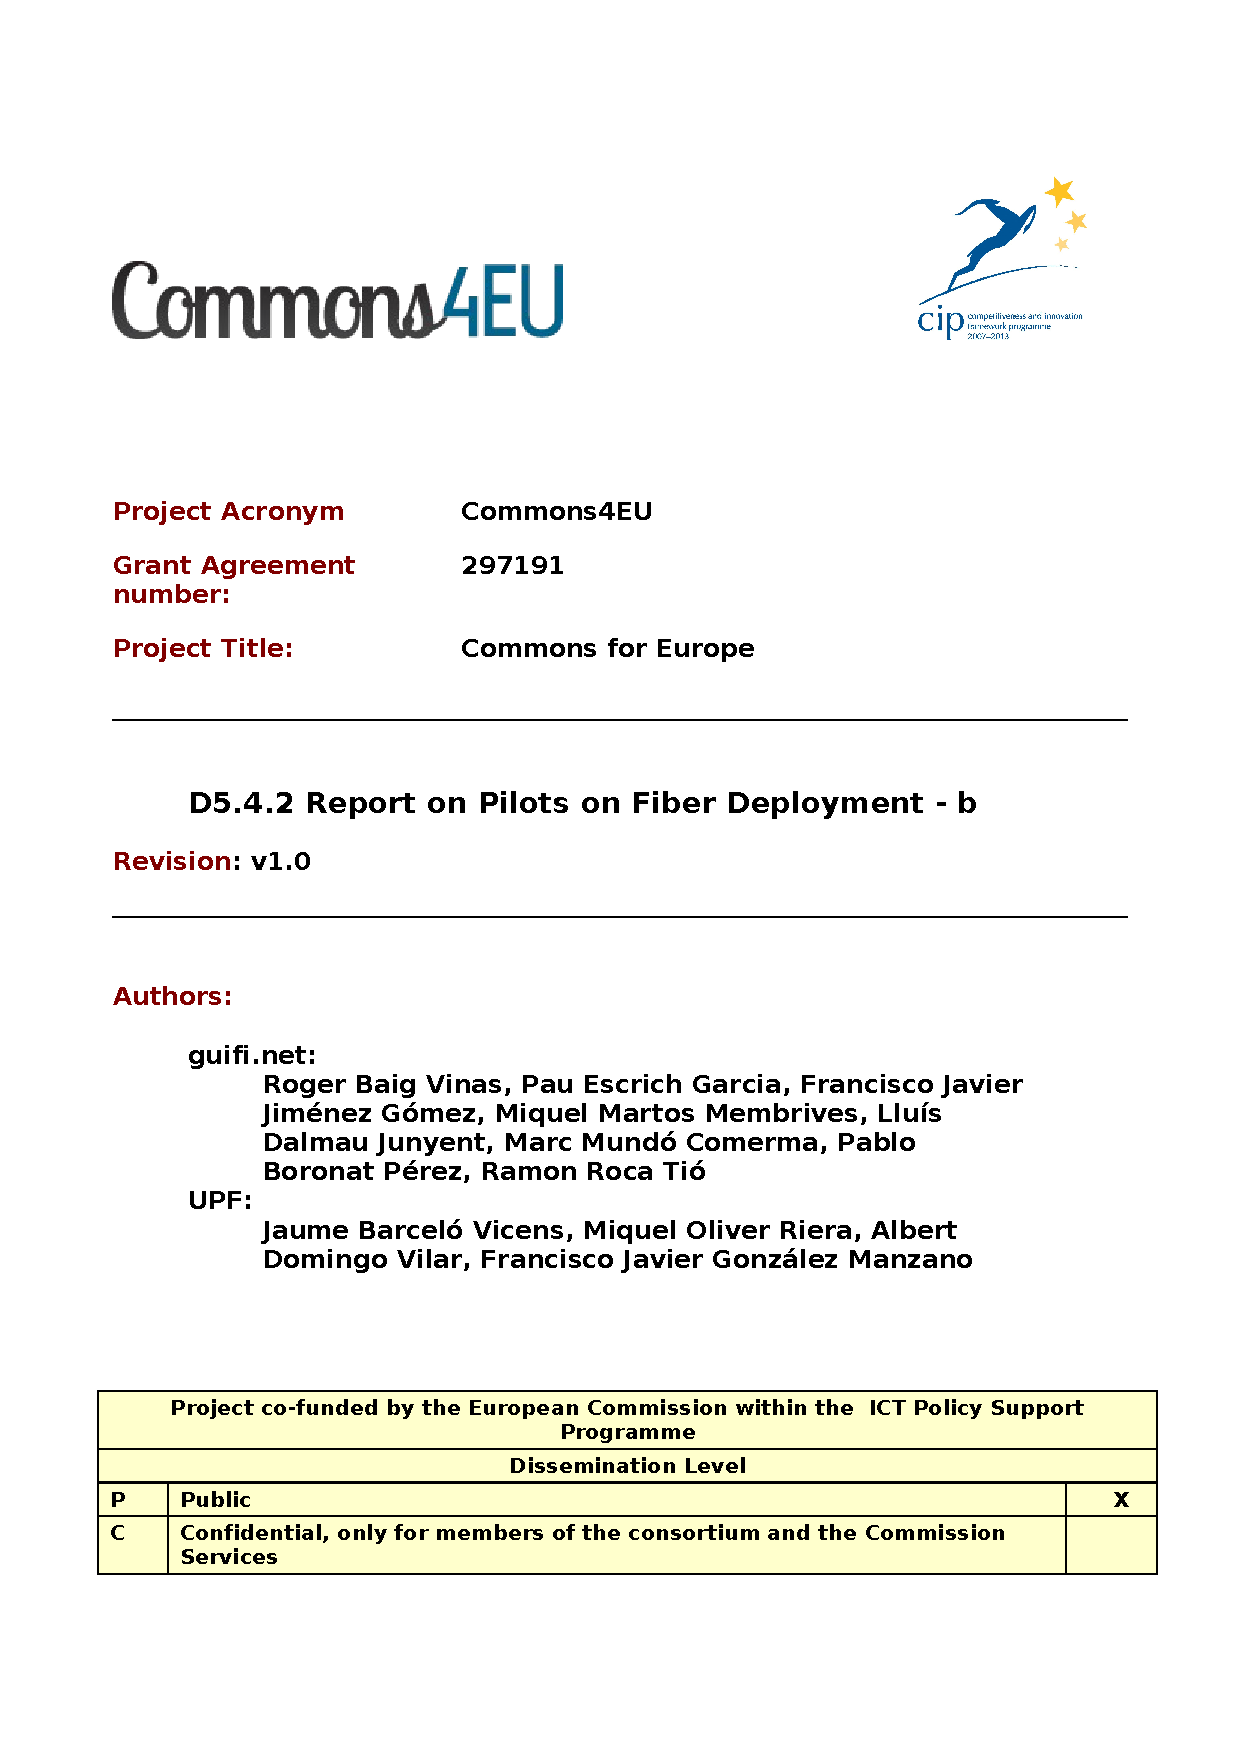
\includepdf[pages=-]{front_cover.pdf}
\thispagestyle{fancy}


\begin{abstract}
%\boldmath
  Optical Fiber is certainly the best technology available for data transmission in terms bandwidth, latency, reliability and stability. As installation costs decrease, it is expanding beyond its original realm and major application in the carrier backbone and is moving into the local loop. Following this trend community networks are gradually adopting it. Thus this technology is one of the three selected in Commons for Europe project for Bottom-Up Broadband pilots. The present technical report accounts for progress made during the second reporting period (Nov 2012 - Oct 2013) of optical fiber pilots in the Commons for Europe project.

  \vspace*{\fill}
\end{abstract}

\vspace*{\fill}

\renewcommand{\abstractname}{Background / Suggested Reading}
\begin{abstract}
%\boldmath
  The socio-economics fundamentals of the optical fiber pilots as long as the technological aspects are explained in the report of the first reporting period (Nov 2011 - Oct 2012). The present document reports only on the progress made during the second year of these pilots following the same structure of the first report. Thus, it is strongly recommended to be familiar with the first year report before reading this one.

  The "Fiber From The Farm (FFTF) \emph{D5.4.1: Report on Pilots on Fiber Deployment -a}" report, the first reporting period report of fiber pilots, can be found at \url{https://github.com/jbarcelo/C4EU-deliverables/blob/master/D_5_4_1_report_on_pilots_on_fiber_deployment_a/DELIVERED_VERSION/D5.4.1%20Report%20on%20pilots%20on%20fiber%20deployment%20-%20a%20guifi.net_DELIVERED_VERSION.pdf}

  \vspace*{\fill}
\end{abstract}

% IEEEtran.cls defaults to using nonbold math in the Abstract.
% This preserves the distinction between vectors and scalars. However,
% if the journal you are submitting to favors bold math in the abstract,
% then you can use LaTeX's standard command \boldmath at the very start
% of the abstract to achieve this. Many IEEE journals frown on math
% in the abstract anyway.


% Note that keywords are not normally used for peerreview papers.
\begin{IEEEkeywords}
  Bottom-up Broadband (BuB), Community Networks (CNs), Fiber From The Farm (FFTF/FFTx), Optical Fiber (OF), Points-of-Presence (POPs)

  \vspace*{\fill}

\end{IEEEkeywords}

\clearpage

\tableofcontents

%\clearpage

\listoffigures

\listoftables

\clearpage




% For peer review papers, you can put extra information on the cover
% page as needed:
% \ifCLASSOPTIONpeerreview
% \begin{center} \bfseries EDICS Category: 3-BBND \end{center}
% \fi
%
% For peerreview papers, this IEEEtran command inserts a page break and
% creates the second title. It will be ignored for other modes.
\IEEEpeerreviewmaketitle



<<<<<<< HEAD
\section{Introduction}
\label{sec:intro}
\IEEEPARstart{S}{uper} WiFi is an emerging attempt to make use of the available spectrum in the UHF TV band (between $471.25$ and $863.25$~MHz) for wireless data transmissions. This spectrum availability is the result from the digital switchover of analog TV channels, allowing more TV data to be transmitted over the same $8$~MHz-width UHF TV channel.

Some of the benefits of attempting transmission over these frequencies are longer ranges and better building penetration than in the unlicensed $2.4$ and $5$~GHz bands used by the IEEE~$802.11$ set of protocols. These benefits are followed by strict regulatory and technological challenges regarding the administration of TV White Spaces (TVWS) and cognitive capabilities for incumbent avoidance.

This report assesses some of Super WiFi's technical challenges, specially those related to incumbent detection and avoidance~\cite{shellhammer2009technical}. As a result, an energy detector on the UHF TV band is implemented using the Universal Software Radio Peripheral (USRP) Ettus USRP-E110~\cite{ettusUSRPE110} as a radio front end for embedded applications (see Figure~\ref{fig:usrp_combined}) and the open source Software Defined Radio (SDR) project GNURadio~\cite{GNURadio}. Furthermore, an instant image of the TV UHF band is derived from the detection (see Figure~\ref{fig:tvChannels}).

Section~\ref{sec:related_work} overviews previous work in this area, followed by Section~\ref{sec:implementation} which details the implementation of a spectrum sensor using the USRP-E110. Results are summarized in Section~\ref{sec:results} while conclusions and future directions are provided in Section~\ref{sec:conclusions}.

\section{About this document}
\label{sec:about}
This report has been produced using open source tools such as {\LaTeX} \cite{lamport1994ldp} and \emph{git} \cite{chacon2009pg}.
{\LaTeX} is widely used in academia to prepare print-class documents.
It automatically takes care of numbering, cross-referencing, tables of contents, bibliography, etc.
\emph{Git} is a high performance distributed revision control which is used in many open source projects, such as the linux kernel.
Git makes it easy and safe to collaborate as each contributor works on his or her own personal copy.
Good contributions can be easily shared with others, and it is always possible to revert to a previous version.

Our git repository is publicly available in \emph{github}:

https://github.com/jbarcelo/C4EU-deliverables

Anyone who is familiar with {\LaTeX} and \emph{github} can contribute to this document.
The first step is to make a copy (a \emph{fork} in \emph{github} jargon).
The contributor can work on this copy and make changes to improve the document.
After that, it is necessary to request that these changes are merged into the original copy of the document (a \emph{pull request} in github jargon).

If you see anything that can be improved, feel free to contribute.
This document is alive in the sense that it will keep evolving as long as contributors make changes and improve it.

The system automatically keeps track of all the contributors and their contributions. 
It is possible to see who is contributing more actively and which are the exact changes made by each contributor.
And everything is public on the web.


\section{Related work}
\label{sec:related}
Results of year one of T7.2 were reported at \emph{D7.2.1 Report on activities to enlist BuB organizations - a} and of T7.3 at \emph{D7.3.1 Report on building support for BuB4Europe - a}. \emph{Report on Opportunites \& Best Practices} reported on the results of T7.1, \emph{Analysis of opportunities and best practices}, also carried out during year one.


=======
%\section{Introduction}
%\label{sec:intro}
%\IEEEPARstart{S}{uper} WiFi is an emerging attempt to make use of the available spectrum in the UHF TV band (between $471.25$ and $863.25$~MHz) for wireless data transmissions. This spectrum availability is the result from the digital switchover of analog TV channels, allowing more TV data to be transmitted over the same $8$~MHz-width UHF TV channel.

Some of the benefits of attempting transmission over these frequencies are longer ranges and better building penetration than in the unlicensed $2.4$ and $5$~GHz bands used by the IEEE~$802.11$ set of protocols. These benefits are followed by strict regulatory and technological challenges regarding the administration of TV White Spaces (TVWS) and cognitive capabilities for incumbent avoidance.

This report assesses some of Super WiFi's technical challenges, specially those related to incumbent detection and avoidance~\cite{shellhammer2009technical}. As a result, an energy detector on the UHF TV band is implemented using the Universal Software Radio Peripheral (USRP) Ettus USRP-E110~\cite{ettusUSRPE110} as a radio front end for embedded applications (see Figure~\ref{fig:usrp_combined}) and the open source Software Defined Radio (SDR) project GNURadio~\cite{GNURadio}. Furthermore, an instant image of the TV UHF band is derived from the detection (see Figure~\ref{fig:tvChannels}).

Section~\ref{sec:related_work} overviews previous work in this area, followed by Section~\ref{sec:implementation} which details the implementation of a spectrum sensor using the USRP-E110. Results are summarized in Section~\ref{sec:results} while conclusions and future directions are provided in Section~\ref{sec:conclusions}.
%
%\section{About this document}
%\label{sec:about}
%This report has been produced using open source tools such as {\LaTeX} \cite{lamport1994ldp} and \emph{git} \cite{chacon2009pg}.
{\LaTeX} is widely used in academia to prepare print-class documents.
It automatically takes care of numbering, cross-referencing, tables of contents, bibliography, etc.
\emph{Git} is a high performance distributed revision control which is used in many open source projects, such as the linux kernel.
Git makes it easy and safe to collaborate as each contributor works on his or her own personal copy.
Good contributions can be easily shared with others, and it is always possible to revert to a previous version.

Our git repository is publicly available in \emph{github}:

https://github.com/jbarcelo/C4EU-deliverables

Anyone who is familiar with {\LaTeX} and \emph{github} can contribute to this document.
The first step is to make a copy (a \emph{fork} in \emph{github} jargon).
The contributor can work on this copy and make changes to improve the document.
After that, it is necessary to request that these changes are merged into the original copy of the document (a \emph{pull request} in github jargon).

If you see anything that can be improved, feel free to contribute.
This document is alive in the sense that it will keep evolving as long as contributors make changes and improve it.

The system automatically keeps track of all the contributors and their contributions. 
It is possible to see who is contributing more actively and which are the exact changes made by each contributor.
And everything is public on the web.

%
%\section{Related work}
%\label{sec:related}
%Results of year one of T7.2 were reported at \emph{D7.2.1 Report on activities to enlist BuB organizations - a} and of T7.3 at \emph{D7.3.1 Report on building support for BuB4Europe - a}. \emph{Report on Opportunites \& Best Practices} reported on the results of T7.1, \emph{Analysis of opportunities and best practices}, also carried out during year one.

%
>>>>>>> rbaig/master
\section{Deployments}
\label{sec:deployments}
This section presents the evolution of optical fibre (OF) deployments, from the Points-Of-Presence (POPs) to the end users. POPs are covered in Section~\ref{sec:POPs}.

\subsection{Pilot's deployments}
\label{dep_pilots}

During the second reporting period\footnote{NOTE: Commons for Europe project has three reporting periods: Nov 2012 - Oct 2013, Nov 2012 - Oct 2013 and Nov 2013 - Oct 2014. In this document they can also be referred as fist year (Y1), second year (Y2) and third year (Y3), or simply 2012, 2013 and 2014.}, \emph{Gurb}'s pilot, the most developed of the three pilots, has kept growing steadily in terms of new users connected, in \emph{Vic}'s the PoP has been raised and the initial connections have been made, and in \emph{Rub\'{i}}, a pilot categorised as "blocked" by the end of the first year, new opportunities for the third year have appeared.


\FloatBarrier

\subsubsection{Gurb}
\label{dep_gurb}

In the first OF initiative in guifi.net, where the PoP infrastructure had been risen, put into service and the first deployment iteration made even before Commons for Europe project was started, the second iteration, the deployment expected for the second year, is being carried out as planned -three fourths of the users are already connected and the rest are expected to be connected before the end of the year. The two first deployment iterations have proved that the BuB OF model works for rural areas (i.e. farms and isolated houses). This kind of deployments are essentially aerial. On the contrary, the area of third iteration, the third year's iteration, is a urban area (mostly detached houses with seldom apartment buildings). This deployment the wiring will be done mostly using already existing ducts owned by the local government. The terms for their usage have already been established and the agreements signed.

Table~\ref{tab:gurb} summarises the evolution of the \emph{Gurb}'s pilot during the second year. 

\begin{table}[H]\small
  \begin{center}
    \begin{tabular}{|l|c|}
      \hline
      \multicolumn{2}{|c|}{\textbf{OF deployment of \emph{Gurb}'s Pilot in 2013}} \\
      \hline
      \hline
      New users already connected & 40 \\
      \hline
      Additional users expected by the end of 2013 & 20 \\
      \hline
      Unsubscribed users (vs. 2012) & 0 \\
      \hline
      Km of OF deployed & 20 \\
      \hline
    \end{tabular}
    \caption[Gurb pilot: pilot evolution 2013]{Gurb's OF deployment evolution in 2013.}
    \label{tab:gurb}
  \end{center}
\end{table}

Figure~\ref{fig:gurb_2013_detail} shows the deployment evolution on a map. Red are lines existing before 2013. Blue and cyan are end user and backbone lines made operational in 2013. Green are lines to be executed by the end of 2013. Brown are backbone lines planned for 2014.

\begin{figure}[H]
  \centering
<<<<<<< HEAD:D_5_4_2_report_on_pilots_on_fiber_deployment_b/deployments/deployments.tex
    \begin{tabular}{cc}
      \resizebox{70mm}{!}{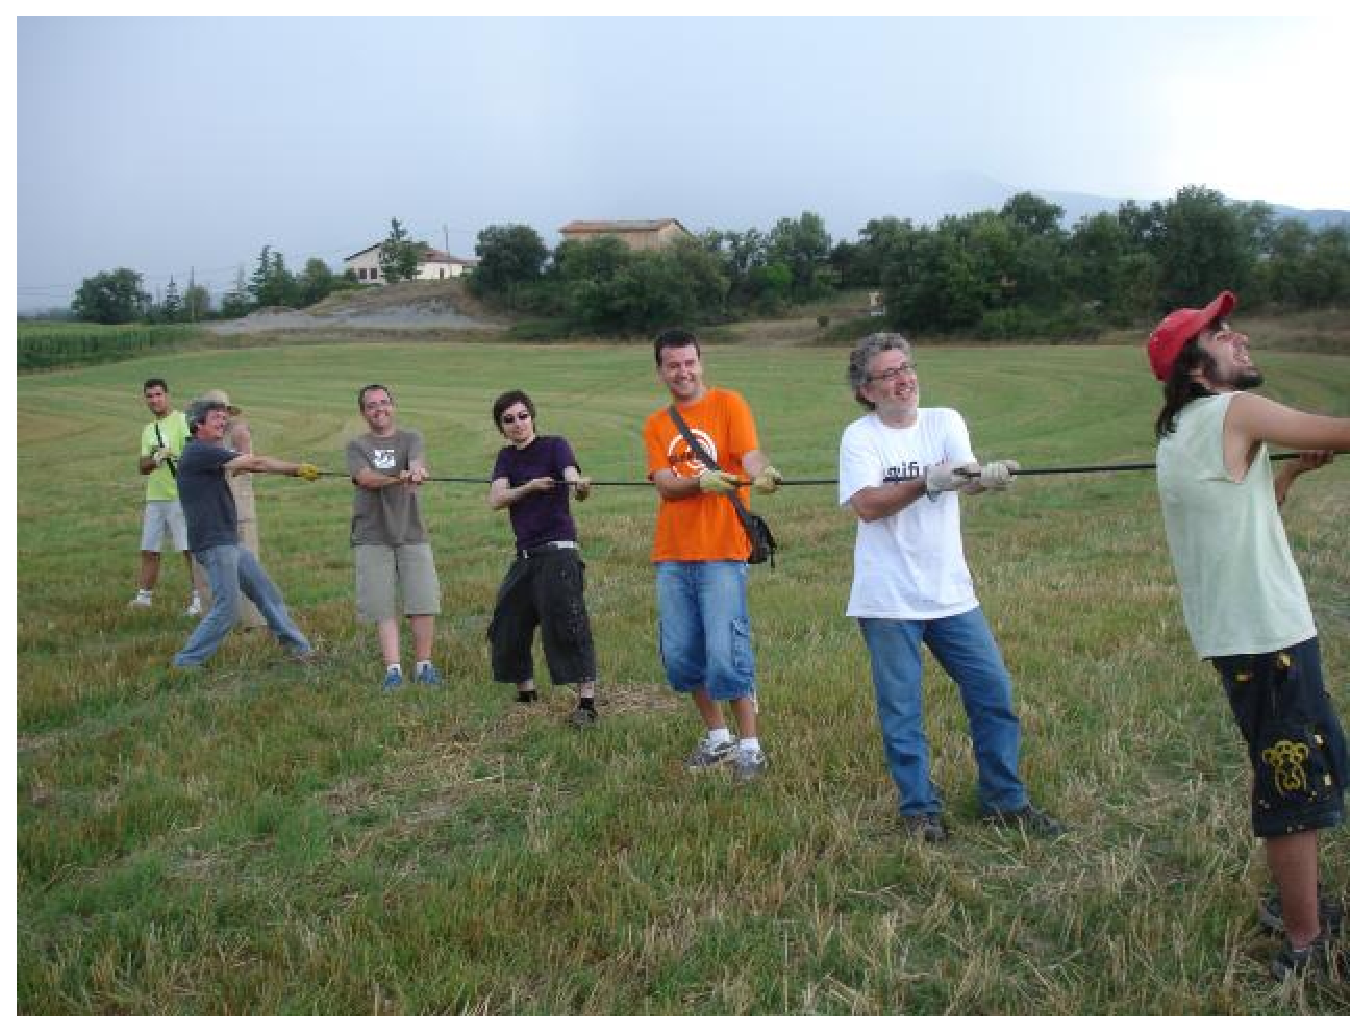
\includegraphics{deployments/figures/Gurb_it1_pic1.eps}} &
      \resizebox{70mm}{!}{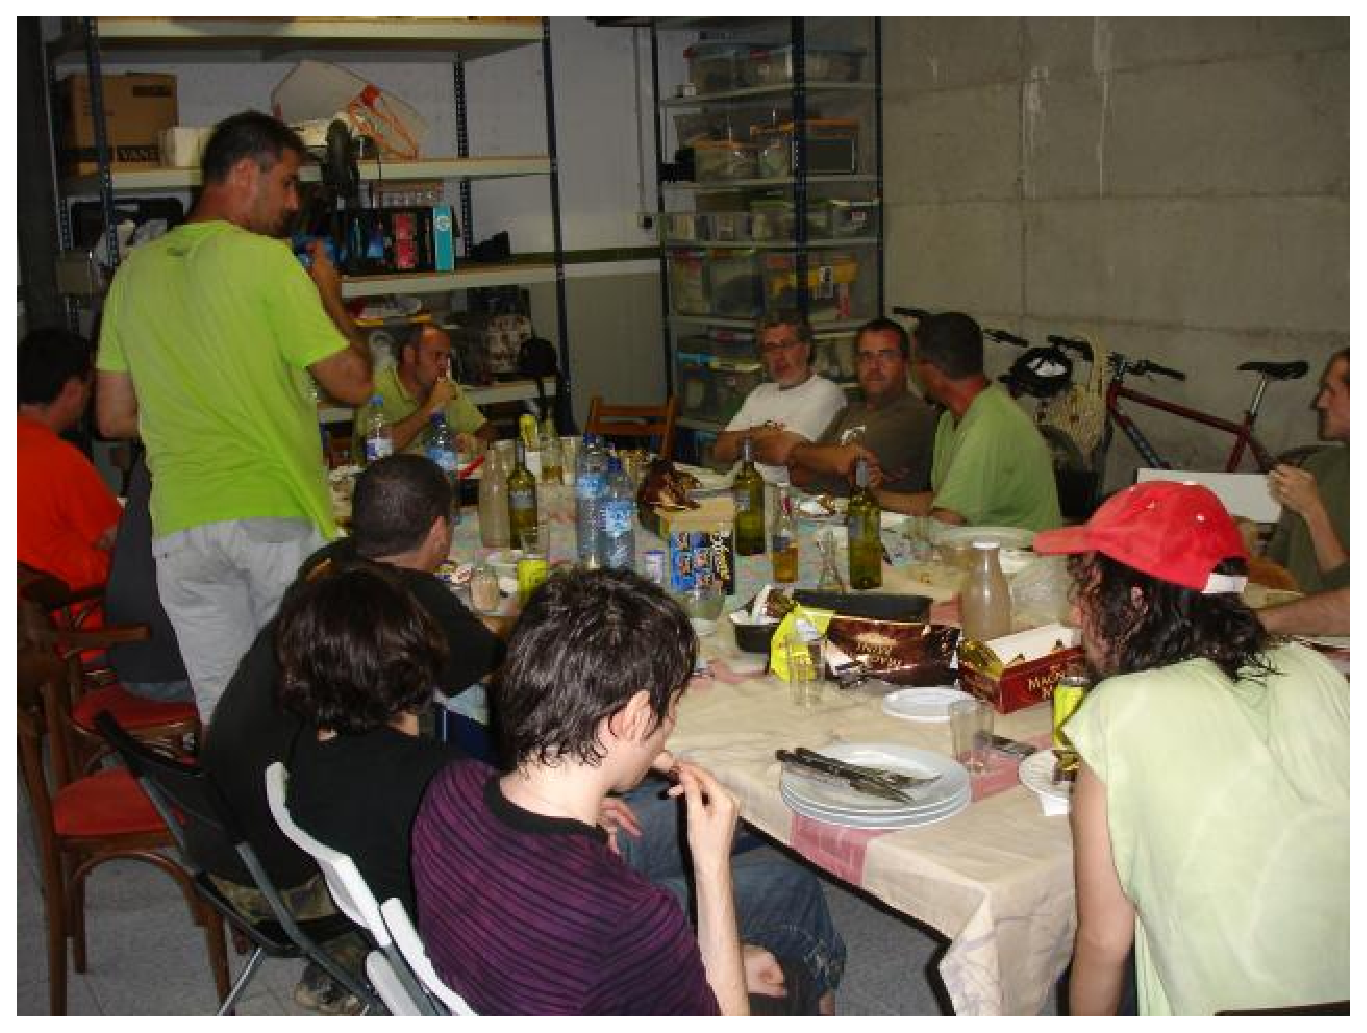
\includegraphics{deployments/figures/Gurb_it1_pic2.eps}} \\
      \resizebox{70mm}{!}{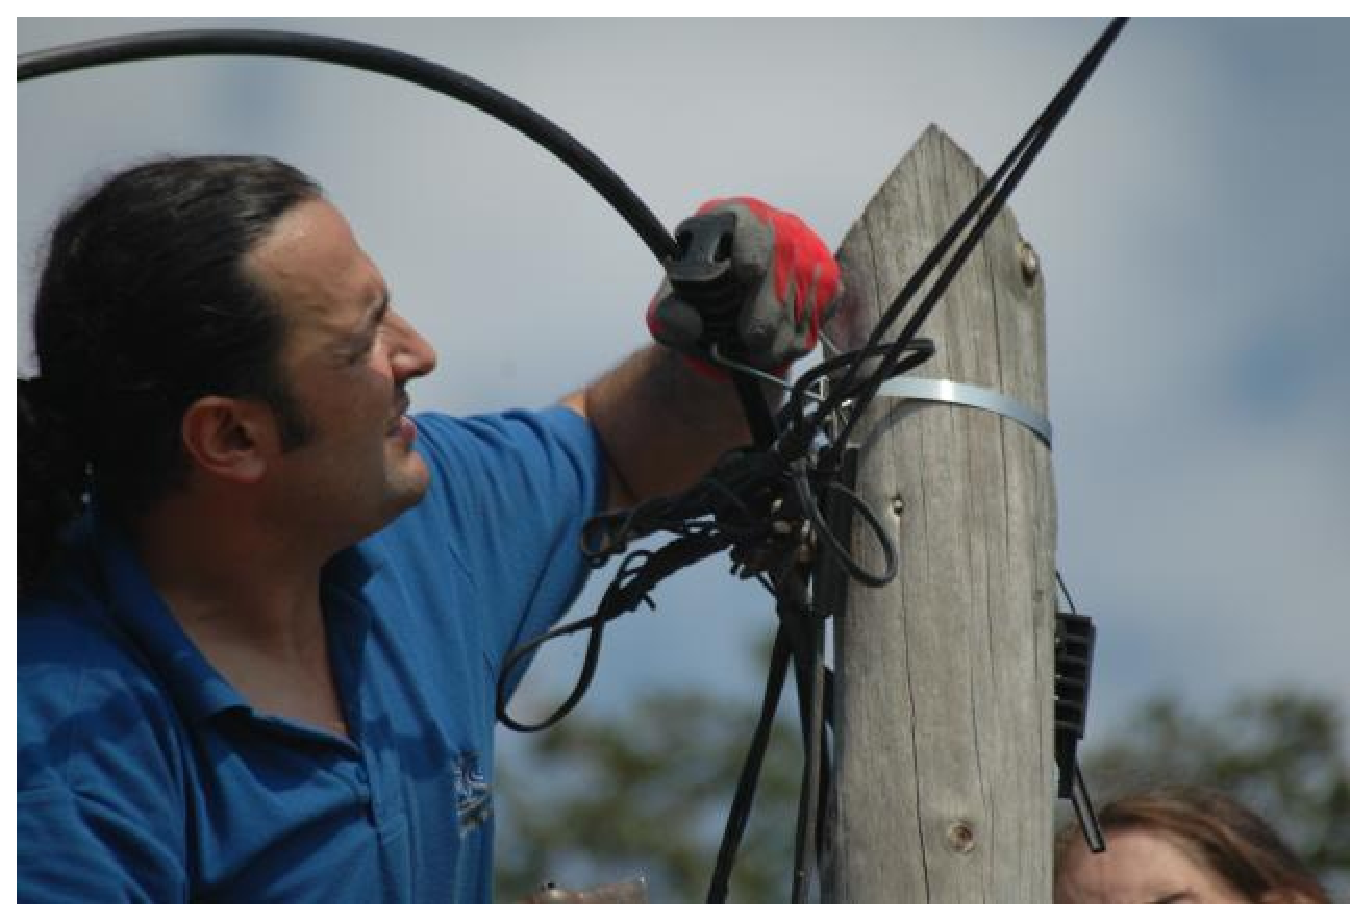
\includegraphics{deployments/figures/Gurb_it1_pic3.eps}} &
      \resizebox{70mm}{!}{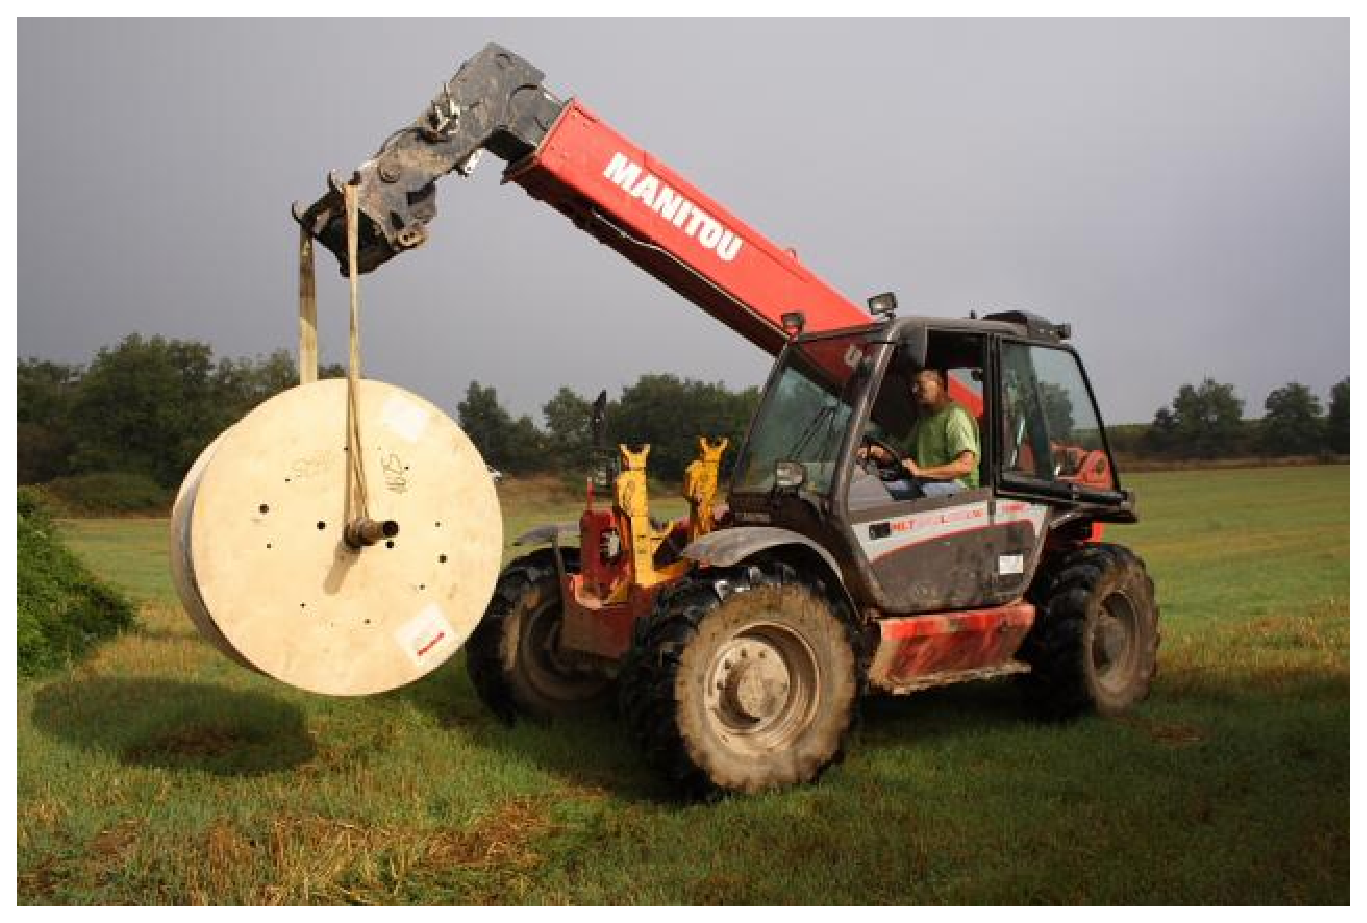
\includegraphics{deployments/figures/Gurb_it1_pic4.eps}} \\
    \end{tabular}
  \caption{OF deployment in Gurb's first iteration. Pictures of the deployment execution, August 2009.}
  \label{fig:gurb_it1_pics}
=======
  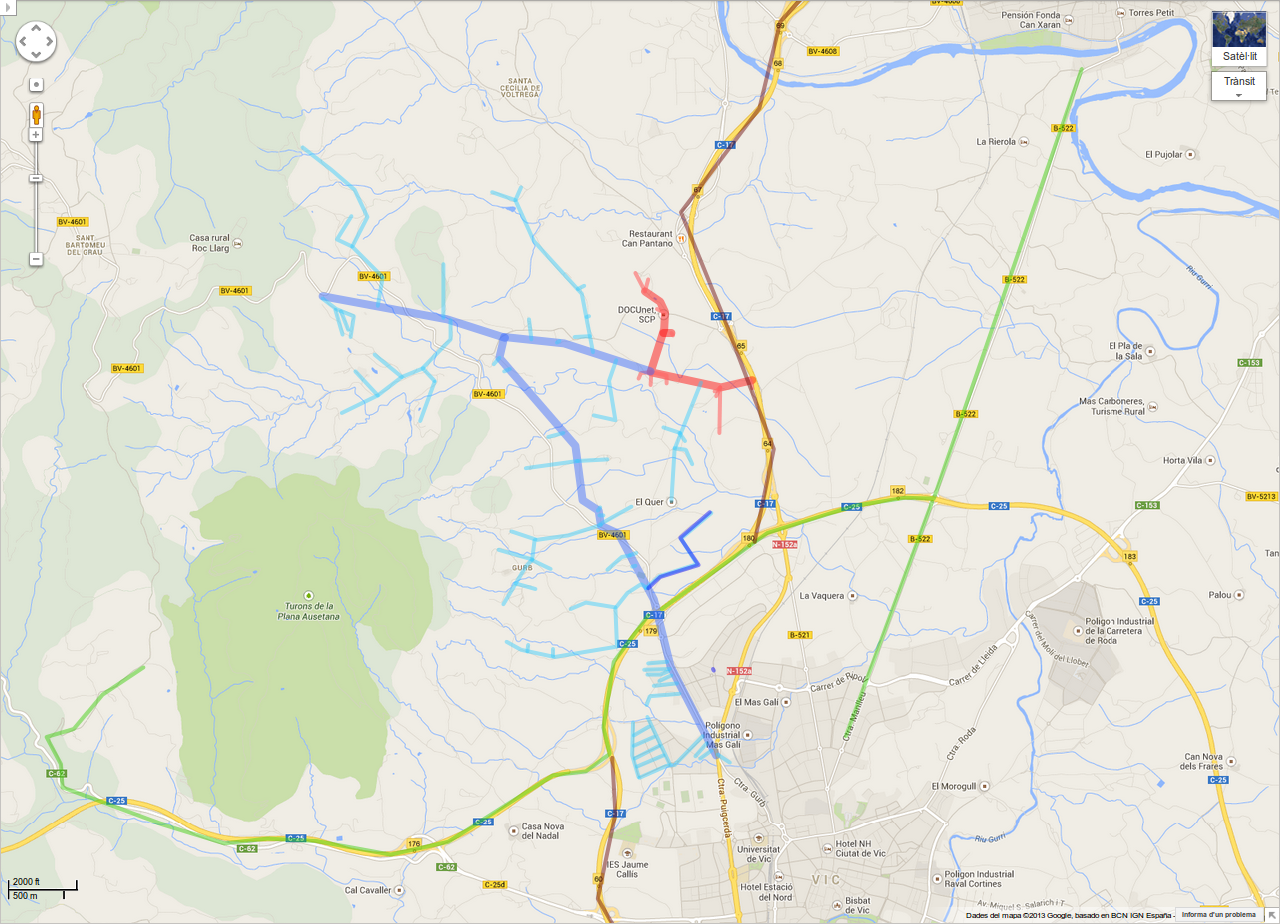
\includegraphics[width=0.95\linewidth]{sect2/figures/gurb_2013_detail.png}
  \caption[Gurb pilot: OF deployment map of 2nd and 3rd iterations]{OF deployment in Gurb's second and third iterations.}
  \label{fig:gurb_2013_detail}
>>>>>>> rbaig/master:D_5_4_2_report_on_pilots_on_fiber_deployment_b/sect2/deployments.tex
\end{figure}

Figure~\ref{fig:gurb_user_con} depicts how end user connections are made.

\begin{figure}[H]
  \centering
<<<<<<< HEAD:D_5_4_2_report_on_pilots_on_fiber_deployment_b/deployments/deployments.tex
  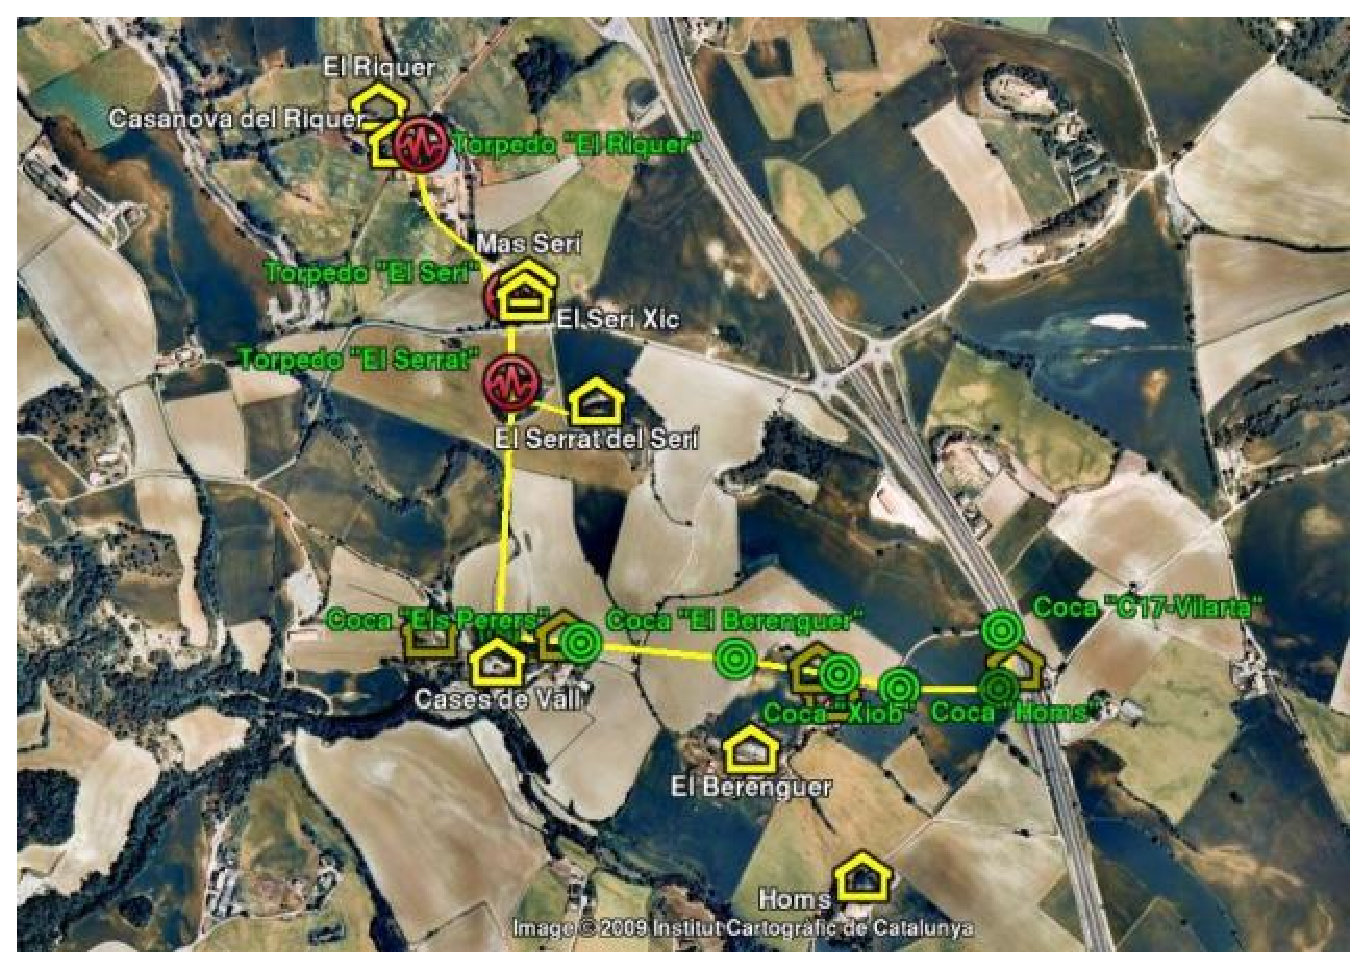
\includegraphics[scale=.65]{deployments/figures/Gurb_it1_map.eps} 
  \caption{OF deployment in Gurb's first iteration. Map. Executed in 2009.}
  \label{fig:gurb_it1_map}
=======
    \begin{tabular}{cc}
      \resizebox{0.465\linewidth}{!}{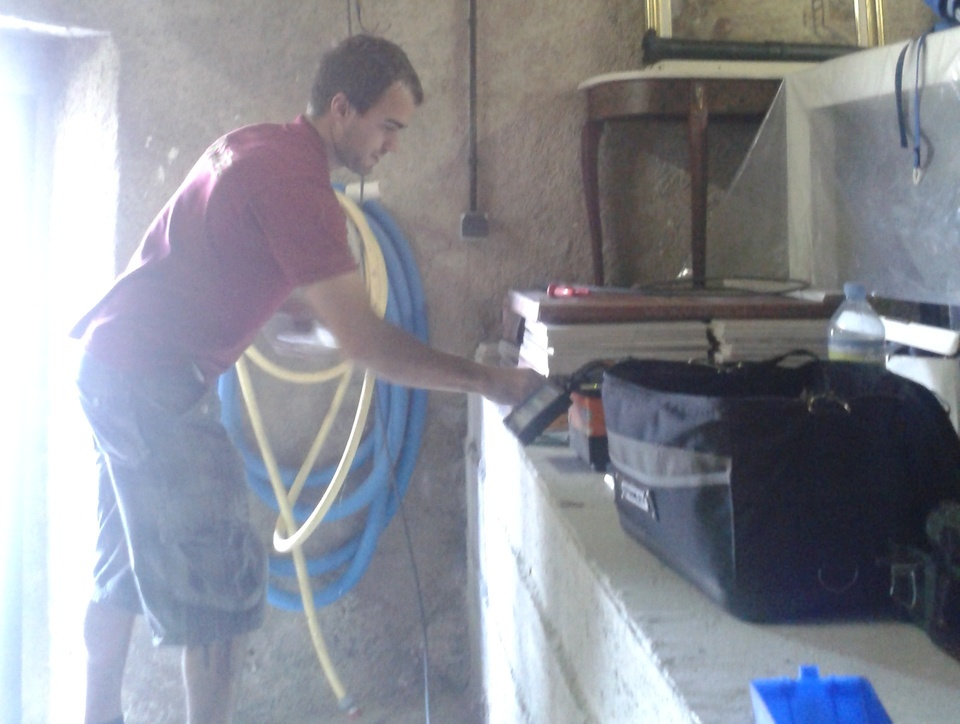
\includegraphics{sect2/figures/user_con1.jpg}} &
      \resizebox{0.465\linewidth}{!}{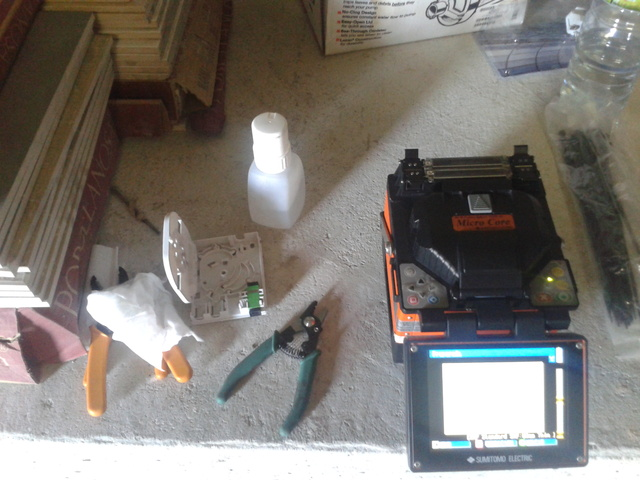
\includegraphics{sect2/figures/user_con2.jpg}} \\
      \resizebox{0.465\linewidth}{!}{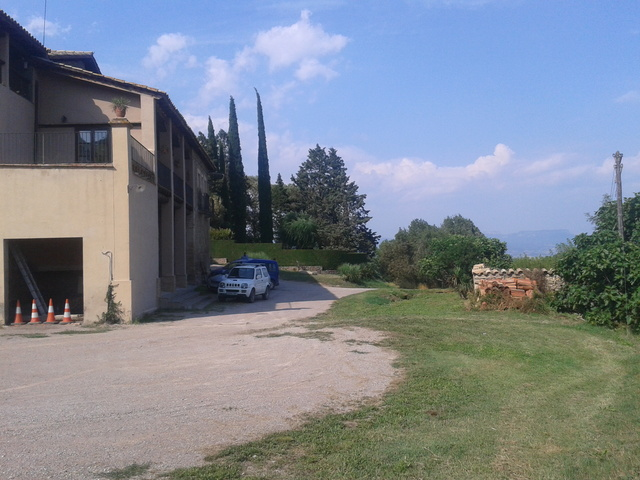
\includegraphics{sect2/figures/user_con3.jpg}} &
      \resizebox{0.465\linewidth}{!}{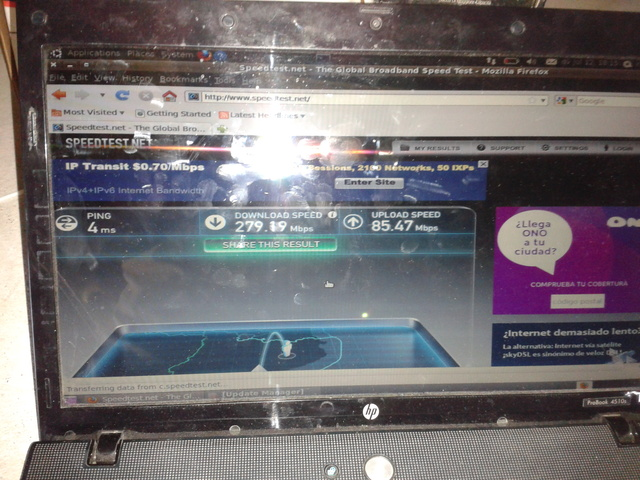
\includegraphics{sect2/figures/user_con4.jpg}} \\
    \end{tabular}
  \caption[Gurb pilot: Connecting a farm]{Connecting a farm. Top left: Preparing the fibre splicer. Top right: The fibre splicer and the additional tools needed. Bottom left: The house being connected. Bottom right: Speed test results.}
  \label{fig:gurb_user_con}
>>>>>>> rbaig/master:D_5_4_2_report_on_pilots_on_fiber_deployment_b/sect2/deployments.tex
\end{figure}

Figure~\ref{fig:gurb_2013_transit} shows the average daily traffic\footnote{All traffic figures are 95-percentile.}. It increases as the number of connected end users increase. The cut of mid September corresponds to a sabotage that took place in September the 11th\footnote{September the 11th is the Catalan national day. It is suspected that the sabotage was directly related to this fact as part of the reaction of the independence process of Catalonia.}.

\begin{figure}[H]
  \centering
<<<<<<< HEAD:D_5_4_2_report_on_pilots_on_fiber_deployment_b/deployments/deployments.tex
  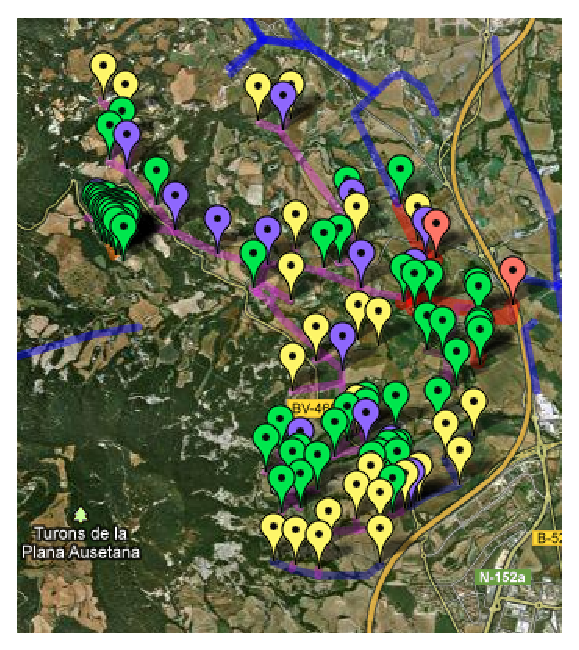
\includegraphics[scale=1.3]{deployments/figures/Gurb_it2_map.eps} 
  \caption{OF deployment in Gurb's fist iteration. Map. Blue spots are the \emph{Passive Optical Splitters}, green spots are homes connected as of the beginning of December 2012, yellow spots are homes to be connected by the end of this iteration.}
  \label{fig:gurb_it2_map}
=======
  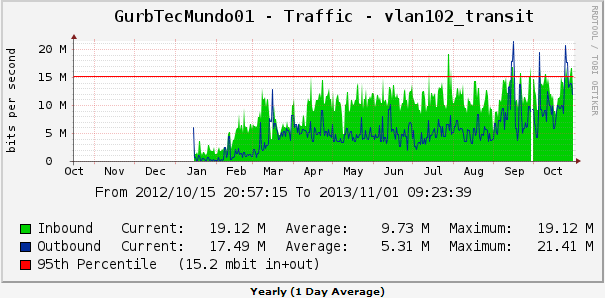
\includegraphics[width=0.95\linewidth]{sect2/figures/gurb_2013_transit.png}
  \caption[Gurb pilot: Network traffic 2013]{Gurb's pilot network traffic 2013.}
  \label{fig:gurb_2013_transit}
>>>>>>> rbaig/master:D_5_4_2_report_on_pilots_on_fiber_deployment_b/sect2/deployments.tex
\end{figure}


\FloatBarrier
\subsubsection{Vic}
\label{dep_vic}

This urban deployment is the result of the collaboration of individuals, industries and social services. In the first iteration a primary and a secondary school, a hospital and chemical industry together with a dozen of dwelling houses have been connected. It is expected that the number of connections will significantly increase in 2014.

Figure~\ref{fig:vic_2013_detail} is the map of the second (2013) and the third (2014) iterations. Green are end user and backbone lines already operational. Orange are lines to be executed by the end of 2013. Red are lines planned for 2014.

\begin{figure}[H]
  \centering
<<<<<<< HEAD:D_5_4_2_report_on_pilots_on_fiber_deployment_b/deployments/deployments.tex
    \begin{tabular}{cc}
      \resizebox{70mm}{!}{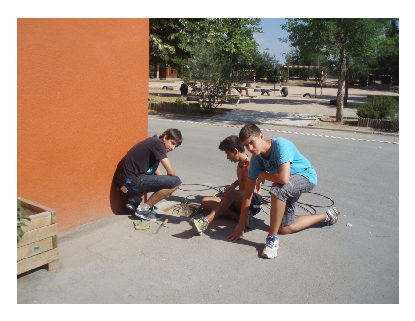
\includegraphics{deployments/figures/Vic_it1_pic1.eps}} &
      \resizebox{70mm}{!}{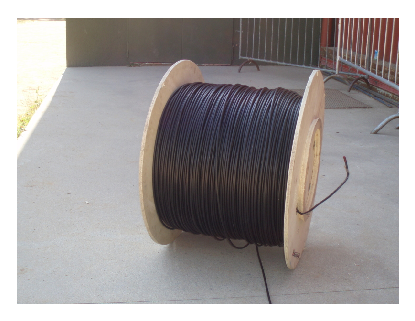
\includegraphics{deployments/figures/Vic_it1_pic2.eps}} \\
      \resizebox{70mm}{!}{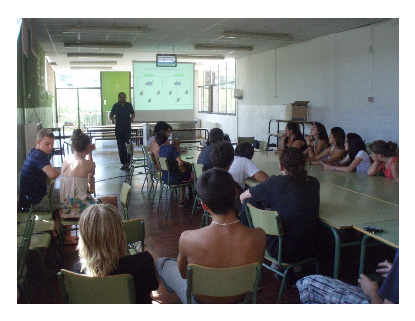
\includegraphics{deployments/figures/Vic_it1_pic3.eps}} &
      \resizebox{70mm}{!}{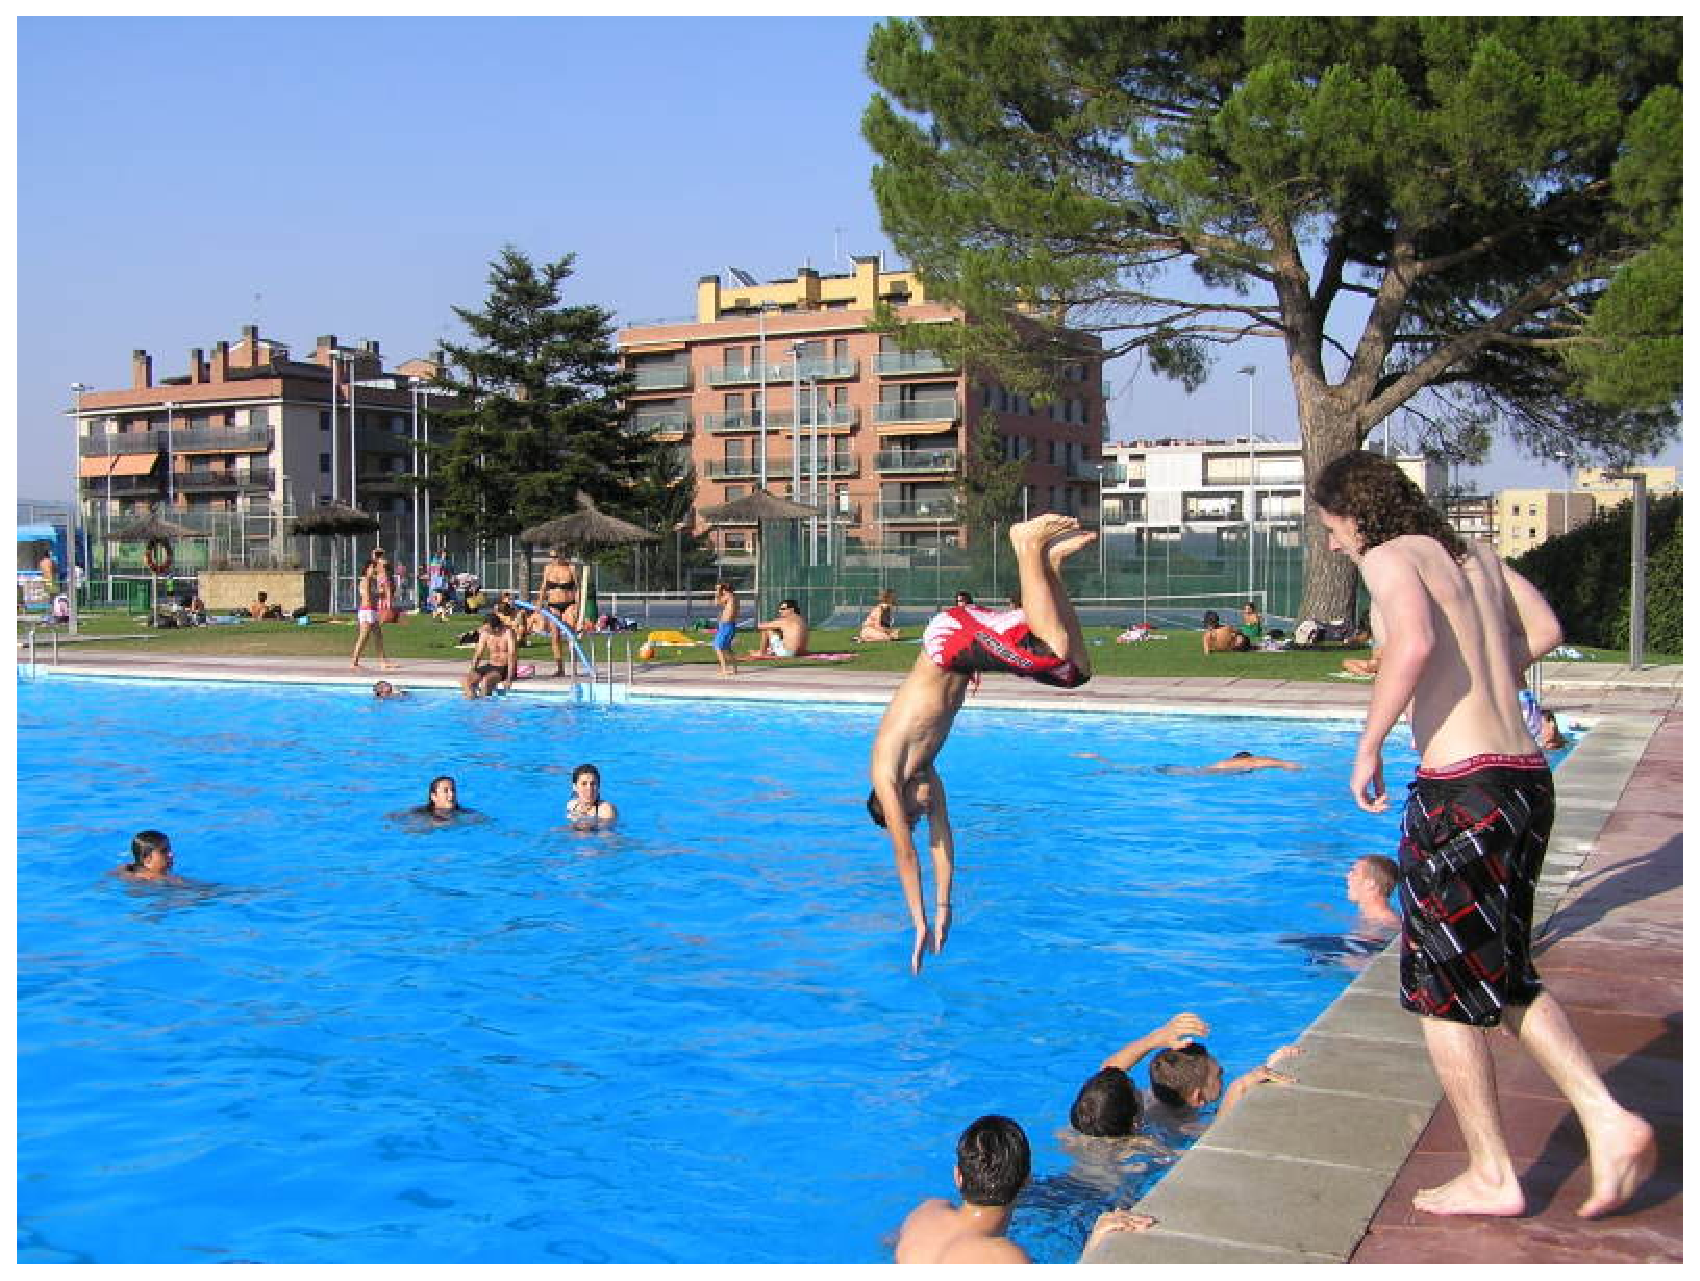
\includegraphics{deployments/figures/Vic_it1_pic4.eps}} \\
    \end{tabular}
  \caption{OF deployment in Vic's first iteration. Pictures of the deployment execution during the summer camp, August 2012.}
  \label{fig:vic_it1_pics}
=======
  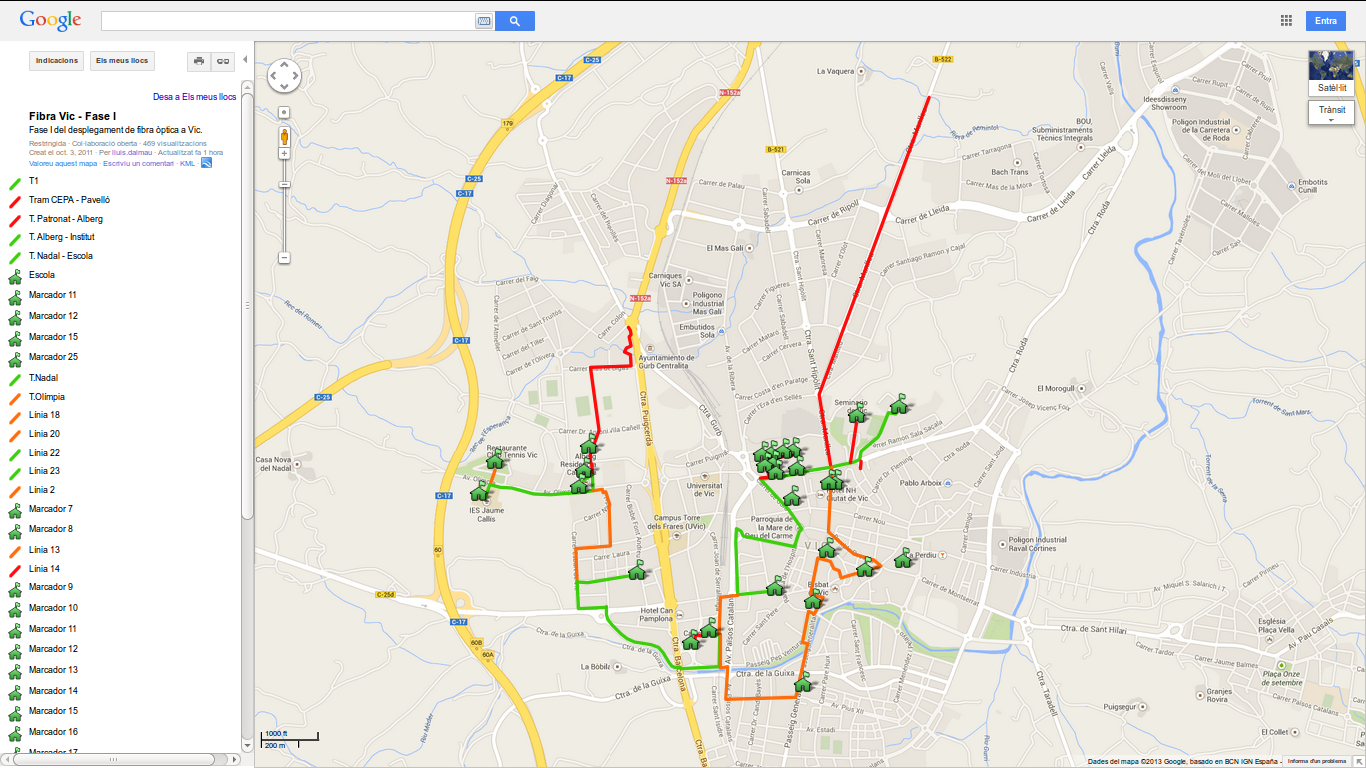
\includegraphics[width=0.95\linewidth]{sect2/figures/vic_2013_detail.png}
  \caption[Vic pilot: OF deployment map of 2nd and 3rd iterations]{OF deployment in Vic's second and third iterations.}
  \label{fig:vic_2013_detail}
>>>>>>> rbaig/master:D_5_4_2_report_on_pilots_on_fiber_deployment_b/sect2/deployments.tex
\end{figure}


\begin{figure}[H]
  \centering
<<<<<<< HEAD:D_5_4_2_report_on_pilots_on_fiber_deployment_b/deployments/deployments.tex
  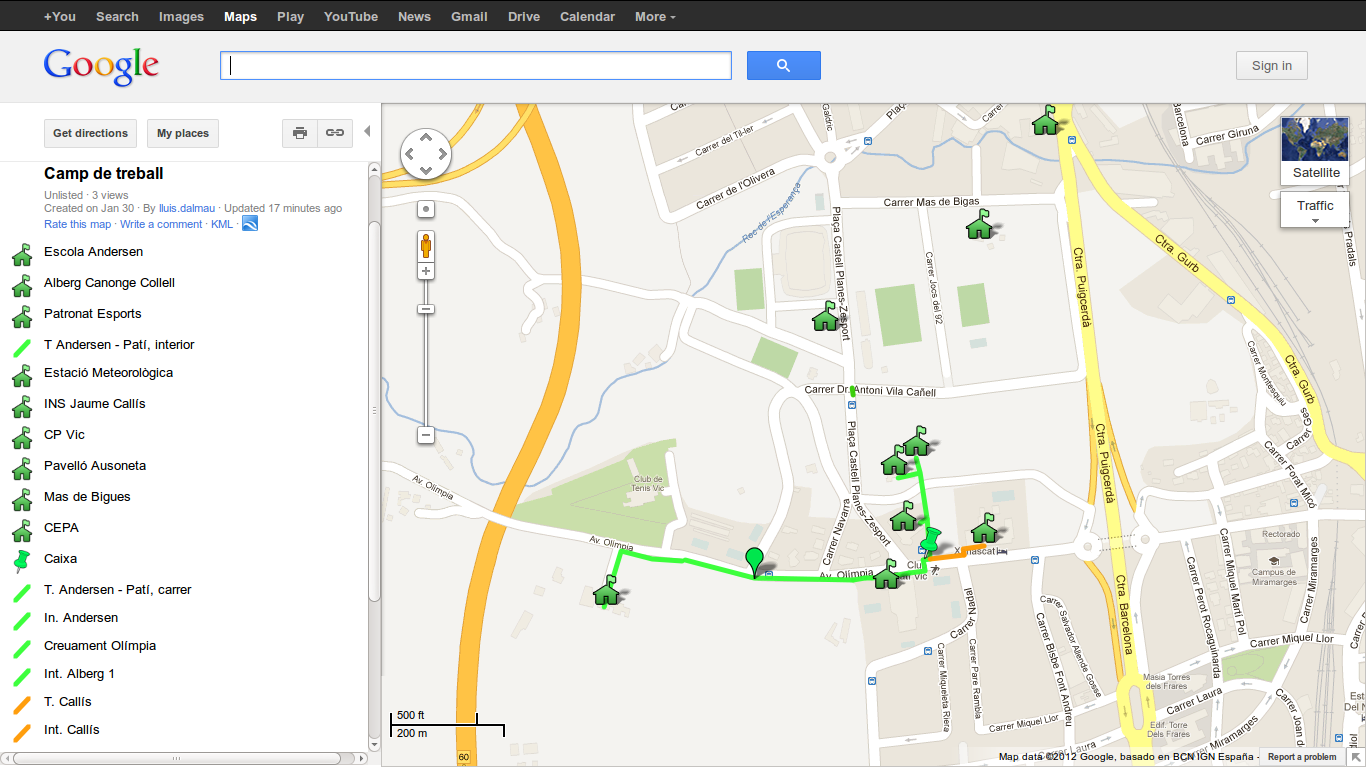
\includegraphics[scale=.33]{deployments/figures/Vic_summer_camp_2012.eps} 
  \caption{OF deployment in Vic's first iteration. Executed in 2012. Result of a teenager's summer camp.}
  \label{fig:vic_sc12}
=======
    \begin{tabular}{cc}
      \resizebox{0.465\linewidth}{!}{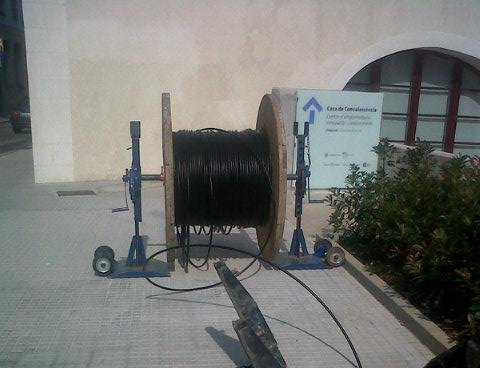
\includegraphics{sect2/figures/20130702_vic_fibra_optica_guifi_net.jpeg}} &
      \resizebox{0.465\linewidth}{!}{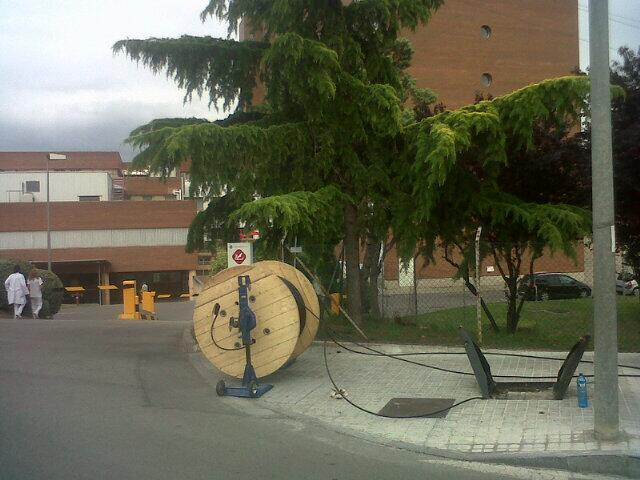
\includegraphics{sect2/figures/20130703_vic_fibra_optica_guifi_net.jpeg}} \\
      \resizebox{0.465\linewidth}{!}{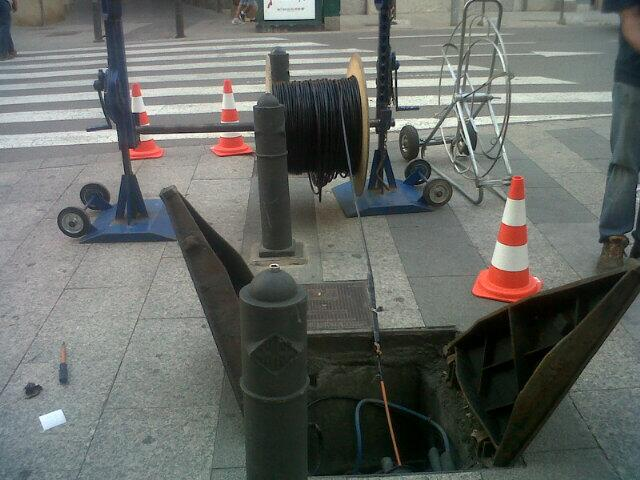
\includegraphics{sect2/figures/20130718_vic_fibra_optica_guifi_net.jpeg}} &
      \resizebox{0.465\linewidth}{!}{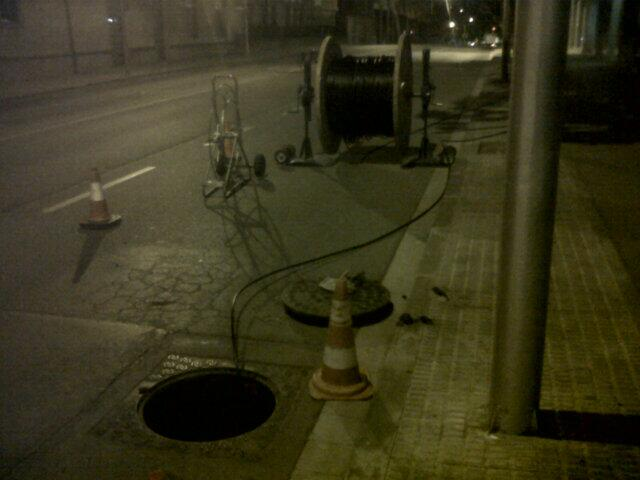
\includegraphics{sect2/figures/20130704_vic_fibra_optica_guifi_net.jpeg}} \\
    \end{tabular}
  \caption[Vic pilot: Connecting a hospital in an urban area]{Connecting a hospital in an urban area. Top left: The fibre reel close to the Hospital's main entrance. Top right: Already outside the Hospital venue. Bottom left: Along the streets. Bottom right: Working until late at night.}
  \label{fig:vic_user_con}
>>>>>>> rbaig/master:D_5_4_2_report_on_pilots_on_fiber_deployment_b/sect2/deployments.tex
\end{figure}


\begin{figure}[H]
  \centering
<<<<<<< HEAD:D_5_4_2_report_on_pilots_on_fiber_deployment_b/deployments/deployments.tex
  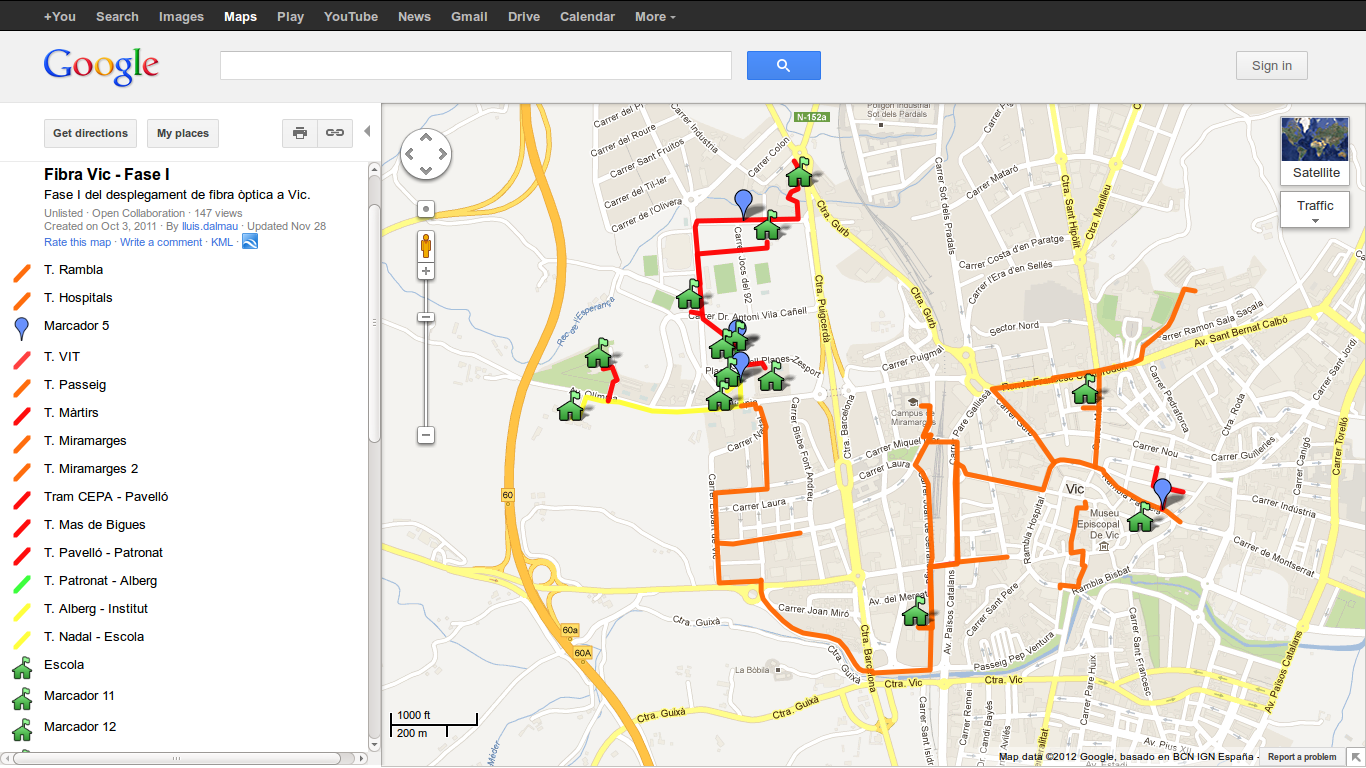
\includegraphics[scale=.33]{deployments/figures/Vic_iteration1.eps} 
  \caption{OF deployment in Vic second iteration. Planned for 2013.}
  \label{fig:vic_it1}
=======
  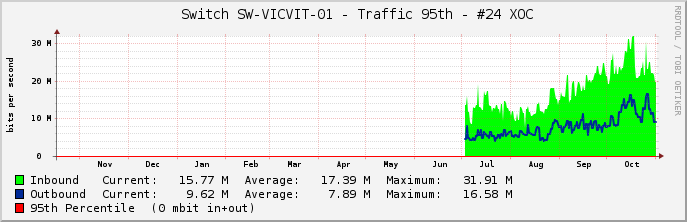
\includegraphics[width=0.95\linewidth]{sect2/figures/vic_2013_transit.png}
  \caption[Vic pilot: Network traffic 2013]{Vic's pilot network traffic 2013.}
  \label{fig:vic_2013_transit}
>>>>>>> rbaig/master:D_5_4_2_report_on_pilots_on_fiber_deployment_b/sect2/deployments.tex
\end{figure}


\FloatBarrier
\subsubsection{Rub\'{i}}
\label{dep_rubi}

As already detailed in the first report, by the end of the first year this pilot was considered to be in a blocked state. In 2013 on the one hand the traditional ISPs have continued deploying their own OF, but on the other hand new opportunities to deploy BuB OF appeared. Indeed, in June a person from the city advised by the local government contacted the guifi.net Foundation to get further information about the BuB model and to discuss on the viability of setting up a consumers cooperative ISP. At the moment it is a work in progress to be consolidated during the year 2014. Nonetheless it looks promising because this person has a wide experience in such kind of cooperatives (she had played a relevant role in the creation of the renewable energies consumer cooperative Som Energia\footnote{\url{http://www.somenergia.coop/welcome-to-som-energia}}) and because the initiative is viewed as favourably by the local government and has its support.


\FloatBarrier
\subsection{Other deployments}
\label{dep_other}

Aside from the selected pilots there are other on-going FO initiatives in side guifi.net at various stages of maturity. The consolidated (those that already have a PoP up and operational) ones are:

\begin{itemize}
\item Masquefa
\item Igualda
\item Manresa
\item Aldea
\item Tortosa
\end{itemize}

<<<<<<< HEAD:D_5_4_2_report_on_pilots_on_fiber_deployment_b/deployments/deployments.tex
% Table~\ref{tab:other_deployments} summarises them.
%
%\begin{table}[htbp]
%  \centering
%    \begin{tabular}{|p{2cm}|p{6cm}|p{6cm}|}
%      \hline \textbf{Project} & \textbf{Status} & \textbf{Comments} \\ \hline \hline
%      Taradell & First iteration executed in 2012 & Interconnection of a secondary school with guifi.net local POP \\
%      Igualda & First iteration planned for 2013 & Connection of many homes expected \\ \hline
%    \end{tabular}
%  \caption{Other deployments.}
%  \label{tab:other_deployments}
%\end{table}
=======
It is expected that other initiatives will consolidate in 2014.
>>>>>>> rbaig/master:D_5_4_2_report_on_pilots_on_fiber_deployment_b/sect2/deployments.tex


\section{Points-Of-Presence (POPs)}
\label{sec:POPs}
During this second year another four territorial PoPs have been raised and made operative, amounting to a total of eight territorial and the concentration one (Telvent -Barcelona) operational. Figure~\ref{fig:pop_weathermap} shows their distribution on the map. So far all the territorial PoPs are connected to the concentration one via XOC connections\footnote{The prices can be found at \url{http://www.xarxaoberta.cat/en/prices}.}.

\begin{figure}[H]
  \centering
  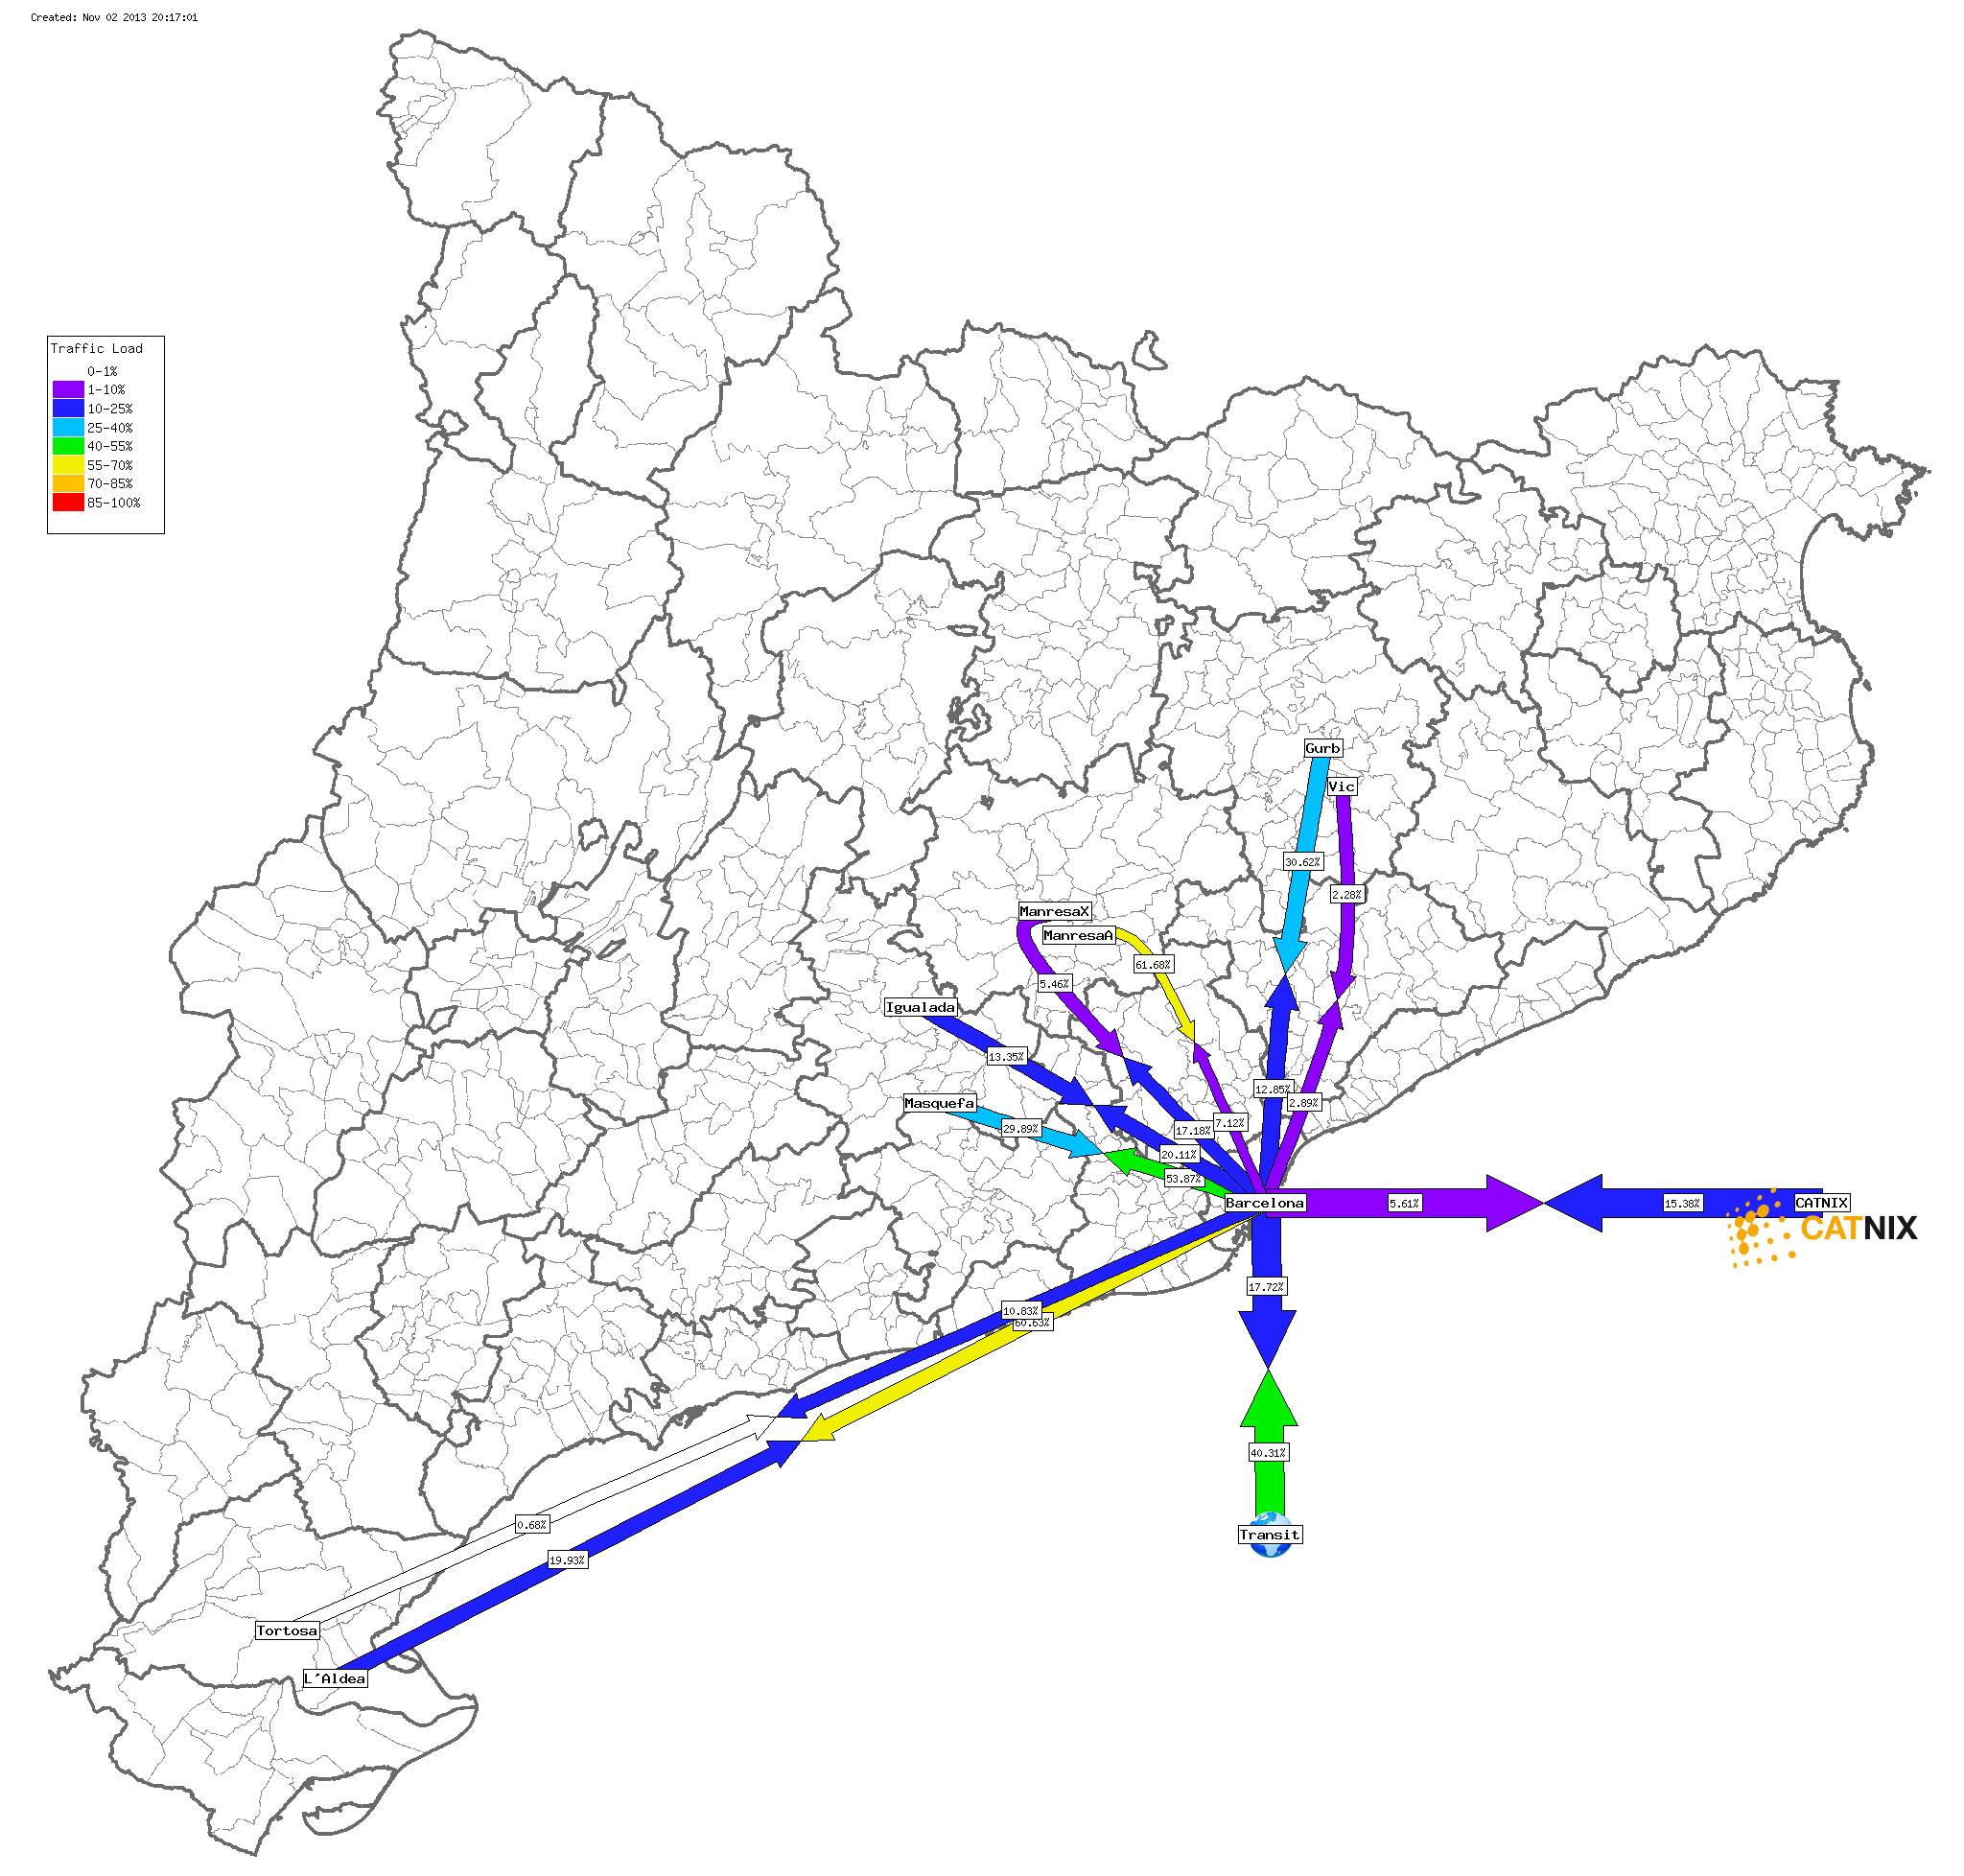
\includegraphics[width=0.95\linewidth]{sect3/figures/weathermap.png} 
  \caption[Guifi.net fiber POPs network map 2013]{Guifi.net fiber POPs network map 2013.}
  \label{fig:pop_weathermap}
\end{figure}

With respect to the IXs operation, the following improvements have been applied during this year:
\begin{itemize}
  \item The management system has been notably enhanced.
  \item A new monitoring development was launched in June 2013 (consequently, most of the traffic graphs shown in the document stars at that moment).
  \item The implementation of a more efficient accounting system has been started and it is expected to be fully operational in 2014. This system will make the ISPs' theshowback/chargeback more accurate and fair.
  \item The equipment of most of the PoPs has been completed and updated.
\end{itemize}

As an example of the current state of the art of the PoPs Figure~\ref{fig:telvent_diagram} shows Telvent's PoP at wiring level.

\begin{figure}[H]
  \centering
  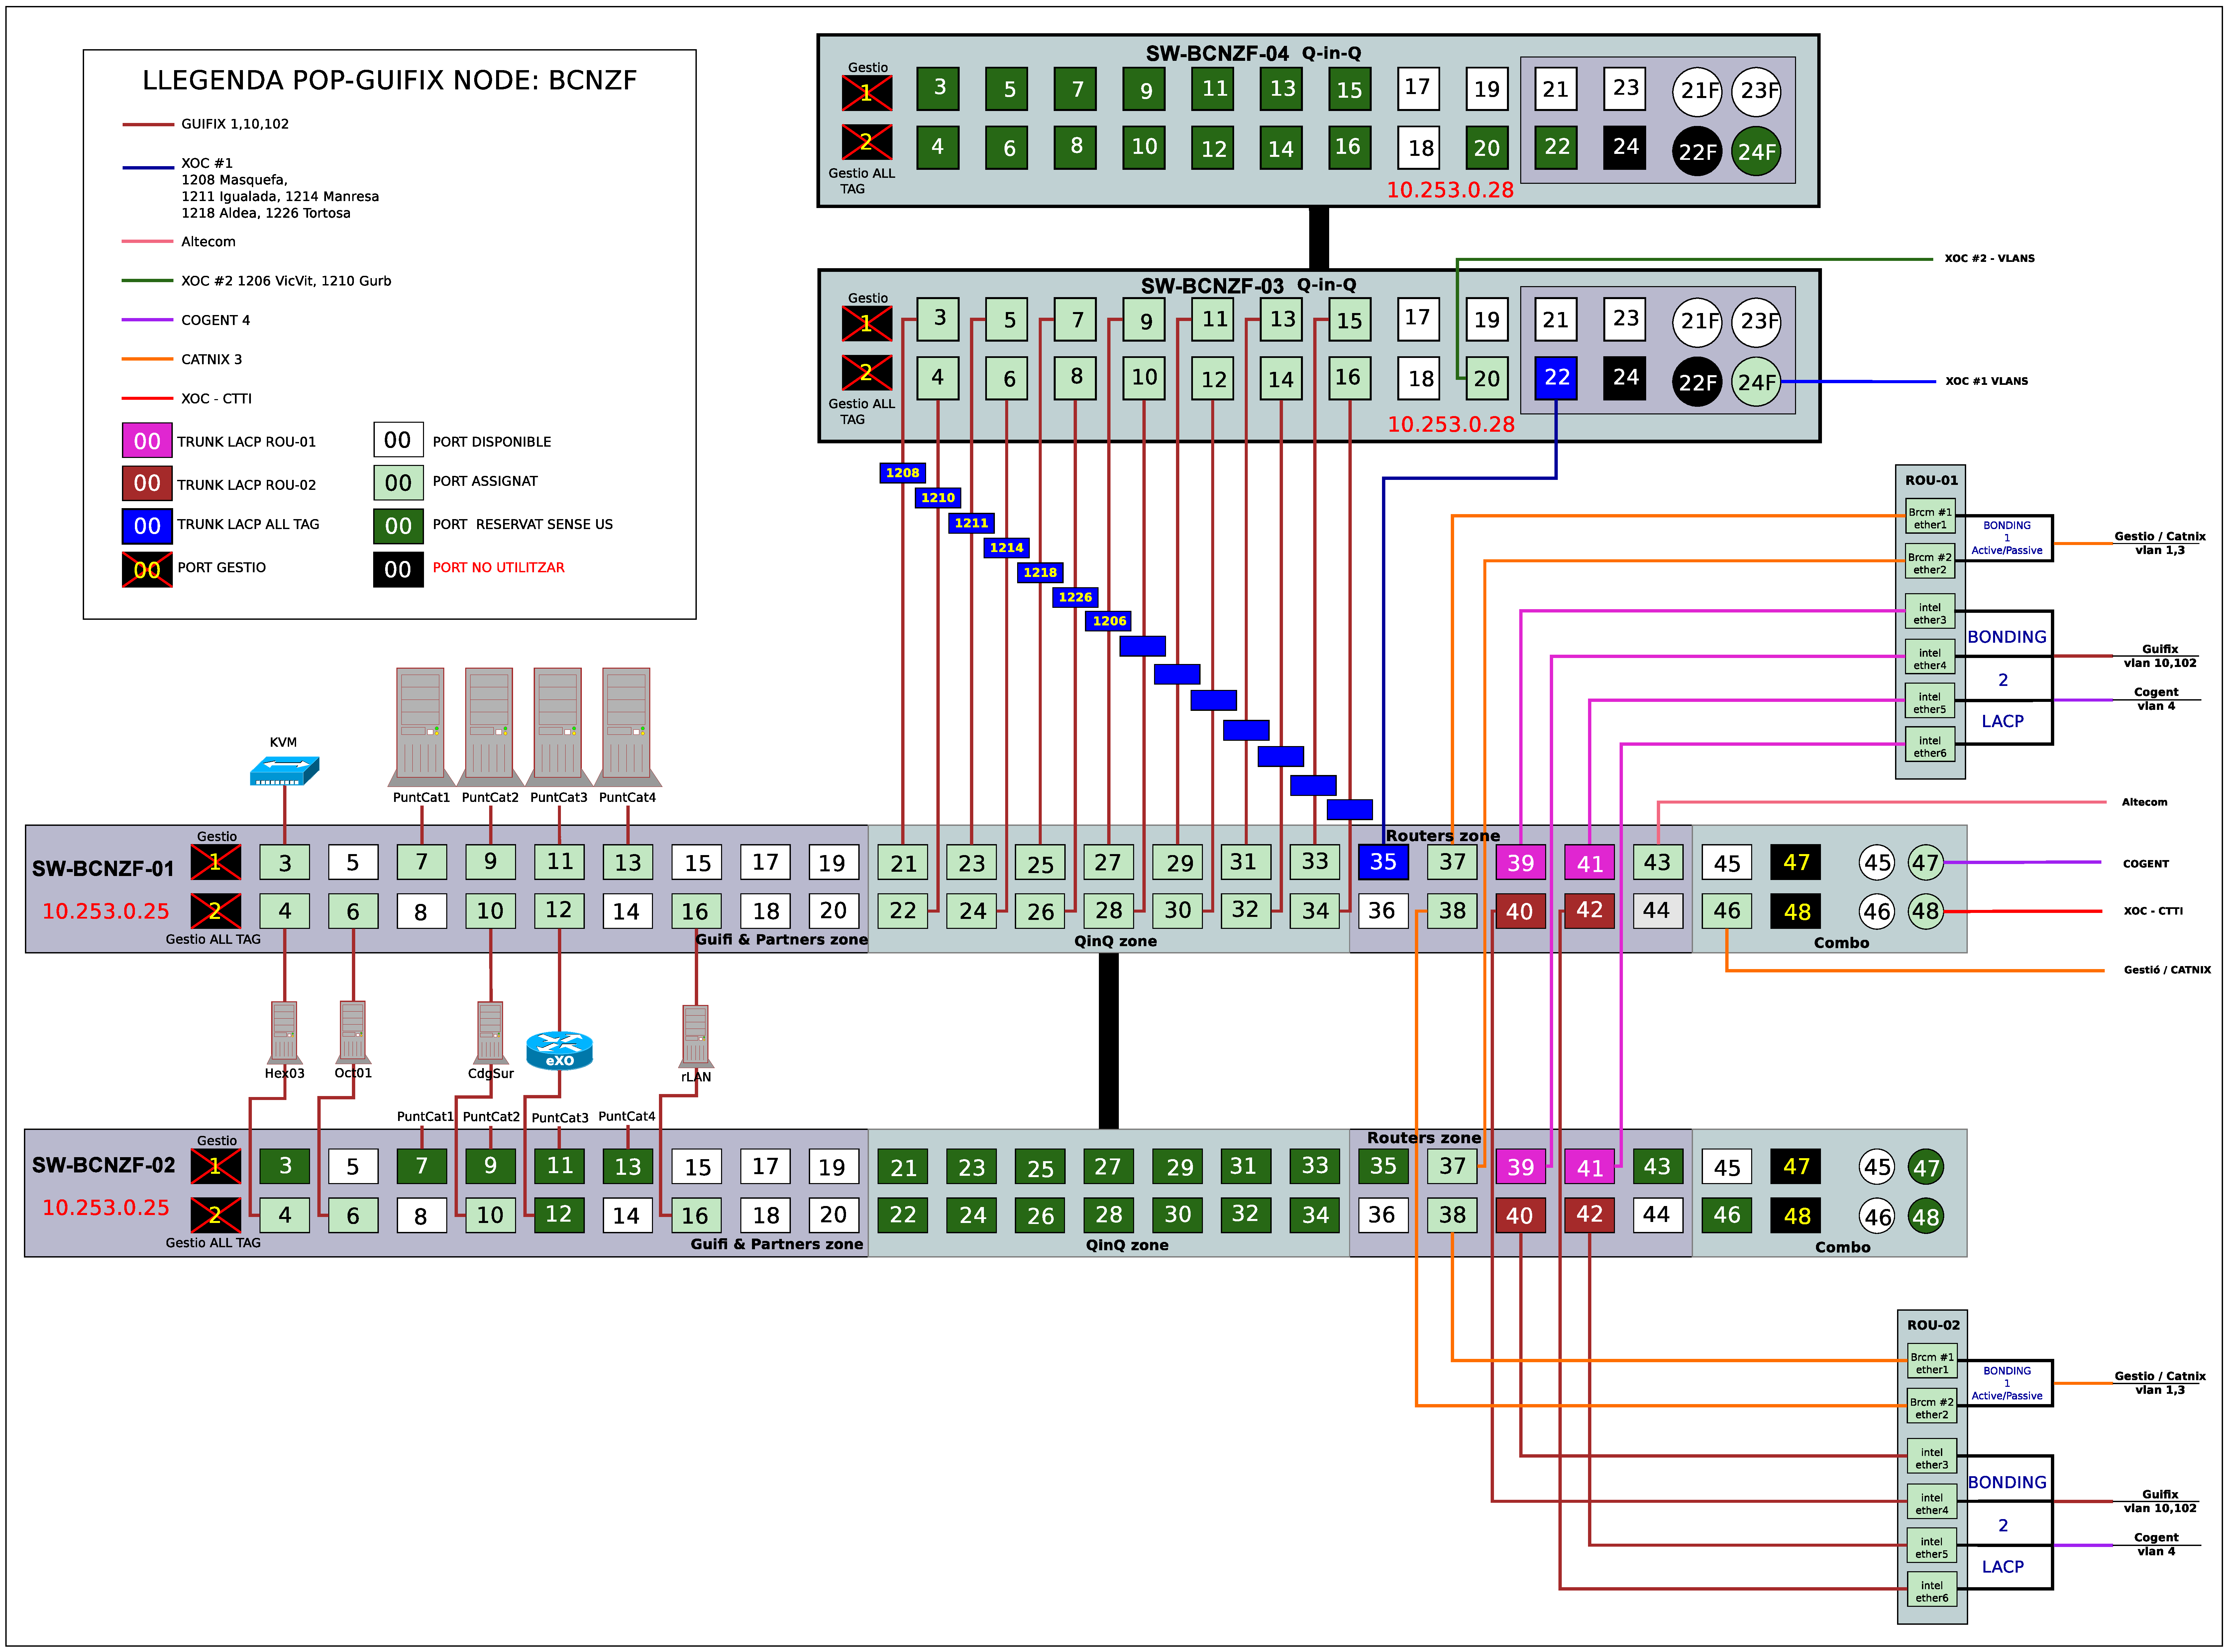
\includegraphics[width=0.95\linewidth]{sect3/figures/telvent_diagram.eps} 
  \caption[Telvent network diagram]{Telvent network diagram Oct. 2013.}
  \label{fig:telvent_diagram}
\end{figure}


During this period the CATNIX (the Catalan exchange point) peering process has been completed. As a result, the guifi.net Foundation is peering with all the other CATNIX members with the exception of the big ISPs (the Telefonica -the incumbent, Ono and BT). These ISPs have not shown any interest in peering with us.

Figure~\ref{fig:catnix_transit} shows the evolution of the peering traffic and Figure~\ref{fig:cogent_transit} shows the traffic to Cogent (our internet carrier). A second carrier is expected to be hired in the coming weeks, essentially to have a redundant internet access but also to anticipate the bandwidth demand.

\begin{figure}[H]
  \centering
  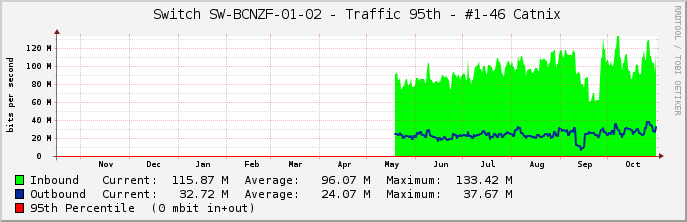
\includegraphics[width=0.95\linewidth]{sect3/figures/catnix.png} 
  \caption[CATNIX traffic 2013]{CATNIX traffic 2013.}
  \label{fig:catnix_transit}
\end{figure}

\begin{figure}[H]
  \centering
  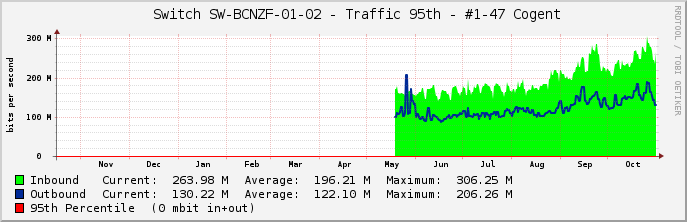
\includegraphics[width=0.95\linewidth]{sect3/figures/cogent.png} 
  \caption[Cogent traffic 2013]{Cogent traffic 2013.}
  \label{fig:cogent_transit}
\end{figure}

\FloatBarrier
\subsection{Pilot's POPs}
\label{pop_pilots}


\FloatBarrier
\subsubsection{Gurb}
\label{pop_gurb}

This PoP has been operative since 2010. This year the power supply system has been improved by adding a back-up power supply. Also the electronic equipment has been significantly extended to accommodate the necessities deriving from Gurb's OF pilot deployment and other connections. Firgure~\ref{fig:gurb_transit} shows the transit of this PoP.

\begin{figure}[H]
  \centering
  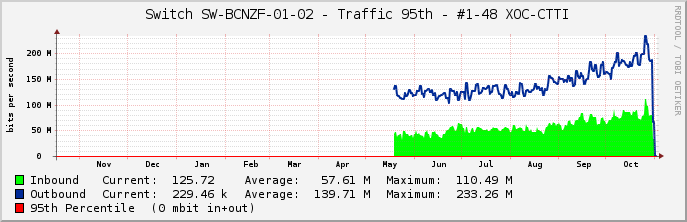
\includegraphics[width=0.95\linewidth]{sect3/figures/gurb.png} 
  \caption[Gurb PoP traffic 2013]{Gurb PoP traffic 2013.}
  \label{fig:gurb_transit}
\end{figure}


\FloatBarrier
\subsubsection{Vic}
\label{pop_vic}

As already foreseen in the previous report, this PoP was activated few days after the report was realised. Despite the fact that Vic borders Gurb, This PoP was raised as an alternative to the impossibility of reaching the Gurb's PoP. The equipment is allocated in a data centre of a facilitate of the local government (http://www.vitvic.cat/). Firgure~\ref{fig:vic_transit} shows the transit of this PoP.

\begin{figure}[H]
  \centering
  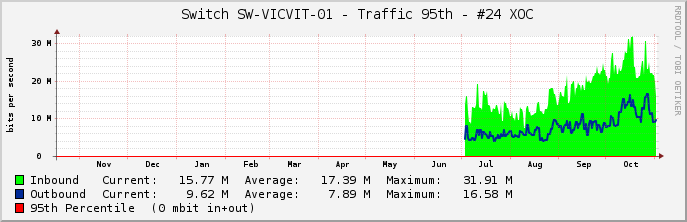
\includegraphics[width=0.95\linewidth]{sect3/figures/vic.png} 
  \caption[Vic PoP traffic 2013]{Vic PoP traffic 2013.}
  \label{fig:vic_transit}
\end{figure}


\FloatBarrier
\subsubsection{Rub\'{i}}
\label{pop_rubi}

In contrast to Vic, where due to its proximity to Gurb the option of not raising a PoP was worked, Rubí pilot clearly needs its own PoP. Thus, if the pilot is eventually developed in 2014 this PoP must be raised.


\FloatBarrier
\subsection{Other POPs}
\label{pop_others}

Firgure~\ref{fig:others_transit} shows the transit of the rest of the operational territorial PoPs .


\begin{figure}[H]
  \centering
    \begin{tabular}{c}
      \resizebox{0.75\linewidth}{!}{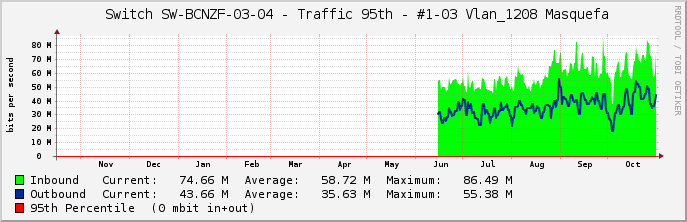
\includegraphics{sect3/figures/masquefa.png}} \\
      \resizebox{0.75\linewidth}{!}{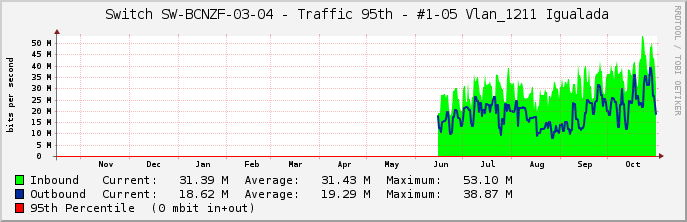
\includegraphics{sect3/figures/igualada.png}} \\
      \resizebox{0.75\linewidth}{!}{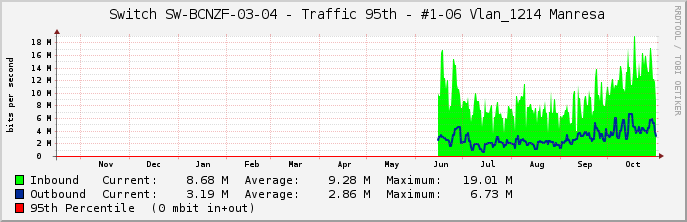
\includegraphics{sect3/figures/manresa.png}} \\
      \resizebox{0.75\linewidth}{!}{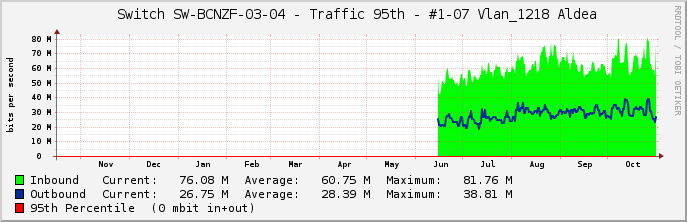
\includegraphics{sect3/figures/aldea.png}} \\
      \resizebox{0.75\linewidth}{!}{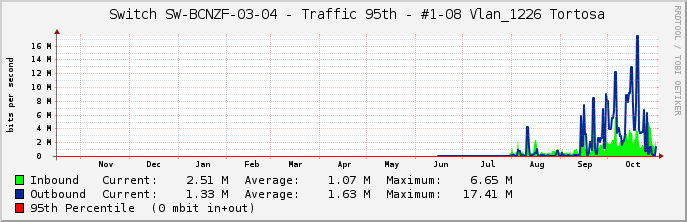
\includegraphics{sect3/figures/tortosa.png}} \\
    \end{tabular}
  \caption[Other PoPs traffic 2013]{Other PoPs traffic 2013. Top: Masquefa. Second top: Igualda. Middle: Manresa. Second bottom: Aldea. Bottom: Tortosa.}
  \label{fig:others_transit}
\end{figure}

%\item Masquefa
%\item Igualda
%\item Manresa
%\item Aldea
%\item Tortosa


\section{Evaluation of Pilot's Results}
\label{sec:results}
We eventually decided not to create a formal organisation as initially planned because we realised that, firstly, there are examples which show that a minimum amount of resources must be committed to an organisation to make it operate properly, and secondly, it was not possible to gather the required commitment to guarantee these resources once the project finished. The comparison of abandoned organisations such as The Open Spectrum Alliance\footnote{At the beginning being this association was very productive and effective in fulfilling its mission, i.e. lobbing the European Commission in favour of allocating more unlicensed electromagnetic spectrum, but once the individual who was doing the vast majority of the work left (at the time of starting the organisation he was unemployed but then he found a job) the activity suddenly ceased and nothing else was done. At the moment, although the domain is registered, the website (\url{http://openspectrum.eu}) has been down for several months.} with active ones such as the Free Software Foundation Europe (FSFE)\footnote{\url{https://fsfe.org/index.en.html}} evidenced that to ensure the success of the organisations these resources, either economic or human, must be in place. In addition, we observed that the general feeling among the practitioners is that the already existing tools such as the International Summit for Community Wireless Netowrks (IS4CWN)\footnote{http://wirelesssummit.org/} and the Wirless Battlem Mesh (WBM)\footnote{http://battlemesh.org/} gathering events and the FNF and guifi.net websites and mailing lists suffice for the coordination among their organizations, and that these tools are adjusted to their realities. The possibility of not creating the formal organisation was already explained during the second review meeting and was accepted by the Project Officer.

During our meetings to investigate about the conscience of the creation of a formal entity to support BuB initiatives we realised that some of the tools we developed during this reporting period (e.g. the English version of the FONN Compact) were, somehow, expected to have already been put in place by guifi. On the contrary, some others such as the economic compensation or the conflicts resolution systems have been received with great expectation and were totally unforeseen.

The Free Network Foudnation has contributed to the translation of the FONN Compact and has integrated its preamble in their license. Now the efforts are put in the translation of the conflicts resolution system. The ITRF GAIA research group\footnote{Global Access to the Internet for All\url{https://trac.tools.ietf.org/group/irtf/trac/wiki/gaia}} has welcomed the guifi.net tools.

In guifi.net, the economic compensation system has already been implemented in 3 PoPIX and it is expected that the rest will adopt it in the coming months. PoPIX set up from now on will include this system since the begining.

Now that the OF as well as the wireless hybrid nodes is supported, the efforts have been focused in registering the already deployed infrastructure.



\section{conclusion}
\label{sec:conclusions}
Work Package 7 of Commons for Europe project aims to support the creation of a pan European organization that could provide structure and support to the existing Bottom-up-Broadband initiatives in Europe from either public organizations or emergent from citizen activism. The present report accounts on the results of task T7.3, \emph{Building Support for BuB4Europe}, achieved during the its first year (second year of the project). 

T7.3 has a strong dependency on the outcome of T7.2, foreseen by the first half of the next year. As a consequence, the activity in T7.3 during this period has been limited at (informally) presenting the initiative to some local administrations and attending some international meeting.

Since T7.2 is being developed according to schedule and suffice resources have been allocated to T7.3 it is expected that this task  as well as WP7 objectives will be fully accomplished by the end of the Commons for Europe.



% The very first letter is a 2 line initial drop letter followed
% by the rest of the first word in caps.
% 
% form to use if the first word consists of a single letter:
% \IEEEPARstart{A}{demo} file is ....
% 
% form to use if you need the single drop letter followed by
% normal text (unknown if ever used by IEEE):
% \IEEEPARstart{A}{}demo file is ....
% 
% Some journals put the first two words in caps:
% \IEEEPARstart{T}{his demo} file is ....
% 
% Here we have the typical use of a "T" for an initial drop letter
% and "HIS" in caps to complete the first word.
%\IEEEPARstart{T}{his} is the introduction blah blah blah blah blah blah blah.
%Blah blah blah blah.
%Blah blah blah blah.
%Blah blah blah blah.

% if have a single appendix:
%\appendix[Proof of the Zonklar Equations]
% or
%\appendix  % for no appendix heading
% do not use \section anymore after \appendix, only \section*
% is possibly needed

% use appendices with more than one appendix
% then use \section to start each appendix
% you must declare a \section before using any
% \subsection or using \label (\appendices by itself
% starts a section numbered zero.)
%


%\appendices
%\section{Proof of the First Zonklar Equation}
%Appendix one text goes here.

% you can choose not to have a title for an appendix
% if you want by leaving the argument blank
%\section{}
%Appendix two text goes here.


% use section* for acknowledgement
\section*{Acknowledgment}

This work has been partially funded by the European Commission (grant CIP-ICT PSP-2011-5).
The views expressed in this technical report are solely those of the authors and do not represent the views of the European Commission.


% Can use something like this to put references on a page
% by themselves when using endfloat and the captionsoff option.
%\ifCLASSOPTIONcaptionsoff
%  \newpage
%\fi



% trigger a \newpage just before the given reference
% number - used to balance the columns on the last page
% adjust value as needed - may need to be readjusted if
% the document is modified later
%\IEEEtriggeratref{8}
% The "triggered" command can be changed if desired:
%\IEEEtriggercmd{\enlargethispage{-5in}}

% references section

% can use a bibliography generated by BibTeX as a .bbl file
% BibTeX documentation can be easily obtained at:
% http://www.ctan.org/tex-archive/biblio/bibtex/contrib/doc/
% The IEEEtran BibTeX style support page is at:
% http://www.michaelshell.org/tex/ieeetran/bibtex/
\bibliographystyle{IEEEtran}
% argument is your BibTeX string definitions and bibliography database(s)
\bibliography{IEEEabrv,my_bib}
%
% <OR> manually copy in the resultant .bbl file
% set second argument of \begin to the number of references
% (used to reserve space for the reference number labels box)
%\begin{thebibliography}{1}

%\bibitem{IEEEhowto:kopka}
%H.~Kopka and P.~W. Daly, \emph{A Guide to \LaTeX}, 3rd~ed.\hskip 1em plus
%  0.5em minus 0.4em\relax Harlow, England: Addison-Wesley, 1999.

%\end{thebibliography}

% biography section
% 
% If you have an EPS/PDF photo (graphicx package needed) extra braces are
% needed around the contents of the optional argument to biography to prevent
% the LaTeX parser from getting confused when it sees the complicated
% \includegraphics command within an optional argument. (You could create
% your own custom macro containing the \includegraphics command to make things
% simpler here.)
%\begin{biography}[{\includegraphics[width=1in,height=1.25in,clip,keepaspectratio]{mshell}}]{Michael Shell}
% or if you just want to reserve a space for a photo:

%\begin{IEEEbiography}{Michael Shell}
%Biography text here.
%\end{IEEEbiography}

% if you will not have a photo at all:
%\begin{IEEEbiographynophoto}{John Doe}
%Biography text here.
%\end{IEEEbiographynophoto}

% insert where needed to balance the two columns on the last page with
% biographies
%\newpage

%\begin{IEEEbiographynophoto}{Jane Doe}
%Biography text here.
%\end{IEEEbiographynophoto}

% You can push biographies down or up by placing
% a \vfill before or after them. The appropriate
% use of \vfill depends on what kind of text is
% on the last page and whether or not the columns
% are being equalized.

%\vfill

% Can be used to pull up biographies so that the bottom of the last one
% is flush with the other column.
%\enlargethispage{-5in}



% that's all folks
\end{document}


